%\documentclass{article}
\documentclass[3p,computermodern,10pt]{elsarticle}
\usepackage{fullpage}
%\usepackage{algorithm,algorithmic}
\usepackage[ruled]{algorithm2e}
\usepackage{algpseudocode}
%\usepackage{cite}
\usepackage[utf8]{inputenc}
\usepackage[english]{babel}
\usepackage{amsthm}
\newtheorem{theorem}{Theorem}[section]
\newtheorem{corollary}{Corollary}[theorem]
\newtheorem{remark}{Remark}[section] 
\usepackage{color}
\usepackage{amsmath}
\usepackage{amsfonts}
\usepackage{mathtools}
\usepackage[titletoc,title]{appendix}
%======
\usepackage{float}
%\usepackage{wrapfig,blindtext}
\usepackage{graphicx} % to include images
\usepackage{epstopdf} % to convert eps to pdf
\usepackage{caption}[font=small,skip=-2pt]
\usepackage{subcaption}[font=small,skip=-2pt]
\usepackage{pdfpages}
\usepackage{comment}

\usepackage{hyperref}
\hypersetup{
    colorlinks=true,
    linkcolor=blue,
    filecolor=magenta,      
    urlcolor=cyan,
}
\urlstyle{same}
%\setlength{\belowcaptionskip}{-5pt}
%\usepackage{sfmath} 

\usepackage{tikz}
\usetikzlibrary{positioning, fit, arrows.meta, shapes}
\newcommand{\empt}[2]{$#1^{\langle #2 \rangle}$}
\usetikzlibrary{
  arrows.meta, % for Straight Barb arrow tip
  fit, % to fit the group box around the central neurons
  positioning, % for relative positioning of the neurons
}
\tikzset{
  neuron/.style={ % style for each neuron
    circle,draw,thick, % drawn as a thick circle
    inner sep=0pt, % no built-in padding between the text and the circle shape
    minimum size=3.5em, % make each neuron the same size regardless of the text inside
    node distance=1ex and 2em, % spacing between neurons (y and x)
  },
  group/.style={ % style for the groups of neurons
    rectangle,draw,thick, % drawn as a thick rectangle
    inner sep=0pt, % no padding between the node contents and the rectangle shape
  },
  io/.style={ % style for the inputs/outputs
    neuron, % inherit the neuron style
    fill=gray!15, % add a fill color
  },
  conn/.style={ % style for the connections
    -{Straight Barb[angle=60:2pt 3]}, % simple barbed arrow tip
    thick, % draw in a thick weight to match other drawing elements
  },
}
\numberwithin{equation}{section}

\newcommand{\TODO}[1]{{\color{red}{to do: #1}}}
\newcommand{\timeDummy}{\tau}
\newcommand{\spatialAcronym}{SDR}
\newcommand{\spaceTimeAcronym}{STDR}
\newcommand{\parametricSpaceTimeAcronym}{PSTDR}
\newcommand{\MLSubspaceNameLowercase}{deep subspaces}
%\newcommand{\span}[1]{\text{span}{#1}}
\newcommand{\PSTWeightingMatrix}{\boldsymbol W}
\newcommand{\PSTInnerProduct}[2]{\left( #1, #2 \right)_{*}}
\newcommand{\defeq}{\vcentcolon=}
\newcommand{\RRStar}[2]{\mathbb{V}_{#1}(\RR{#2})}
\newcommand{\Range}[1]{\text{Range}(#1)}
\newcommand{\RomDim}{K}
\newcommand{\NVars}{N_v}
\newcommand{\ParametricSpace}{\mathcal{P}}
\newcommand{\TimeDomain}{[0,T]}
\newcommand{\ParamDomain}{\mathcal{D}}
\newcommand{\paramDomain}{\mathcal{D}}
\newcommand{\numParams}{N_{\mu}}
\newcommand{\numSpaceDims}{N_x}
\newcommand{\SpatialDomain}{\Omega}
\newcommand{\PhysicalDomain}{\Omega}
\newcommand{\PDEStateDomain}{\PhysicalDomain \times \TimeDomain \times \paramDomain}
\newcommand{\PDEStateCodomain}{\RR{\NVars}}
\newcommand{\PDEFlux}{\mathcal{F}}
\newcommand{\NSpace}{N_s}
\newcommand{\NTime}{\numTimeSteps}
\newcommand{\NST}{N_{st}}
\newcommand{\x}{\boldsymbol x}
\newcommand{\xd}{\mathbf{x}}
\newcommand{\xDummy}{\boldsymbol y}
\newcommand{\xs}{x}
\newcommand{\ys}{y}
\newcommand{\zs}{z}
\newcommand{\NeuralNetwork}{\mathcal{NN}}
\newcommand{\TimeSpace}{\mathcal{T}}
\newcommand{\STDim}{K_{\text{st}}}
\newcommand{\PSTDim}{K_{\text{pst}}}

\newcommand{\SemiDiscreteSpaceTimeTrialSpace}{\mathcal{ST}}

\newcommand{\ParametricSpaceTimeTrialSpace}{\mathcal{PXT}}

\newcommand{\SemiDiscreteParametricSpaceTimeTrialSpace}{\mathcal{PST}}

\newcommand{\ParametricSpaceTimeBasisVec}{\boldsymbol \psi}
\newcommand{\ParametricSpaceTimeBasisMat}{\boldsymbol \Psi}

\newcommand{\SpaceTimeBasisVec}{\boldsymbol \pi}
\newcommand{\SemiDiscreteSpaceTimeBasisMat}{\boldsymbol \Pi}
\newcommand{\OnesFunction}{\mathcal{O}}
\newcommand{\SemiDiscreteParametricSpaceTimeBasisMat}{\boldsymbol \Phi}
\newcommand{\SemiDiscreteParametricSpaceTimeBasisVec}{\boldsymbol \phi}

\newcommand{\TrainingData}{\mathcal{S}}
\newcommand{\NTrain}{N_{\text{train}}}
\newcommand{\SemiDiscreteStateIC}{\SemiDiscreteState_0(\params)}
\newcommand{\SemiDiscreteStateParametricSpaceTimeRef}{\SemiDiscreteState_{\text{ref}}}

\newcommand{\RRSym}[1]{\mathbb{R}_{\text{s}}^{#1}}
\newcommand{\RR}[1]{\mathbb{R}^{#1}}
\newcommand{\FomDim}{N}
\newcommand{\ApproxPDEState}{\tilde{\PDEState}}

\newcommand{\PDEStateParametricSpaceTimeTrialSpace}{\textit{PXT}}

\newcommand{\PDEStateSpaceTimeTrialSpace}{\textit{XT}}

\newcommand{\PDEStateSpatialTrialSpace}{\textit{X}}
\newcommand{\SpatialTrialSpace}{\mathcal{X}}
\newcommand{\SpaceTimeTrialSpace}{\mathcal{XT}}

\newcommand{\PDEState}{\mathsf{u}}
\newcommand{\PDEStateRef}{\mathsf{u}_{\text{ref}}}

%\newcommand{\ApproxPDEState}{\tilde{\boldsymbol u}}
\newcommand{\NNWeights}{\boldsymbol \theta}
\newcommand{\NWeights}{N_{\NNWeights}}
\newcommand{\weightsInner}{\boldsymbol \theta^*}
\newcommand{\bz}{\boldsymbol 0}
\newcommand{\params}{\boldsymbol \mu}
\newcommand{\paramsDummy}{\boldsymbol \nu}
\newcommand{\PDEStateArgs}{\x, t,\params}
\newcommand{\weights}{\boldsymbol \theta}
\newcommand{\Basis}{\boldsymbol \Phi}
\newcommand{\SpatialBasisVec}{\boldsymbol \phi}

\newcommand{\BasisVec}{\boldsymbol \phi}
\newcommand{\BasisDiscrete}{\mathbf{\Phi}}
\newcommand{\BasisVecDiscrete}{\mathbf{\boldsymbol \phi}}
\newcommand{\NBasis}{K}
\newcommand{\ApproxPDEStateArgs}{\boldsymbol x, t,\params;\weights}
\newcommand{\GenState}{\hat{\boldsymbol u}}
\newcommand{\BasisArgs}{\boldsymbol x, t,\params;\weightsInner}
\newcommand{\BasisDiscreteArgs}{\params;\weightsInner}
\newcommand{\TrialSpace}{\mathcal{V}}
\newcommand{\velocity}{\boldsymbol f}
\newcommand{\ApproxSemiDiscreteState}{\tilde{\SemiDiscreteState}}
\newcommand{\SemiDiscreteStateRef}{\mathbf{u}_{\text{ref}}}
\newcommand{\SemiDiscreteSpatialTrialSpace}{\mathcal{V}}
\newcommand{\SemiDiscreteSpatialBasisMat}{\mathbf{V}}
\newcommand{\SemiDiscreteSpatialBasisVec}{\mathbf{v}}
\newcommand{\SemiDiscreteGenState}{\hat{\SemiDiscreteState}}
\newcommand{\SemiDiscreteGenStateArgs}{\SemiDiscreteStateArgs}


\newcommand{\FullyDiscreteStateDummy}{\mathbf{v}}

\newcommand{\FullyDiscreteState}{\mathbf{u}}
\newcommand{\FullyDiscreteStateArgs}{\params}

\newcommand{\residLMS}{\boldsymbol{r}}

\newcommand{\CollocationSet}{\mathcal{C}}
\newcommand{\NCollocation}{N_c}
\newcommand{\ResidualLoss}{\mathcal{L}_{r}}

\newcommand{\SemiDiscreteStateDum}{\boldsymbol v}

\newcommand{\SemiDiscreteState}{\boldsymbol u}
\newcommand{\SemiDiscreteStateArgs}{t,\params}
\newcommand{\SpaceTimeGenState}{\overline{\hat{\SemiDiscreteState}}}

\newcommand{\SemiDiscreteSpaceTimeGenState}{\overline{\hat{\SemiDiscreteState}}}
\newcommand{\ParametricSpaceTimeGenState}{\overline{\hat{\SemiDiscreteState}}}
\newcommand{\SemiDiscreteParametricSpaceTimeGenState}{\overline{\hat{\SemiDiscreteState}}}
\newcommand{\SemiDiscreteParametricSpaceTimeGenStateNN}{\overline{\hat{\boldsymbol z}}}
\newcommand{\ParametricSpaceTimeGenStateNN}{\overline{\hat{\boldsymbol z}}}

\newcommand{\DiscreteResid}{\mathbf{R}}
\newcommand{\DiscreteState}{\mathbf{u}}
\newcommand{\DiscreteStateArgs}{\params}
\newcommand{\numTimeSteps}{N_t}
\newcommand{\DiscreteSpaceTimeState}{\overline{\DiscreteState}}
\newcommand{\DiscreteSpaceTimeResid}{\overline{\DiscreteResid}}
\newcommand{\DiscreteSpaceTimeResidArgs}{\params}

\newcommand{\DiscreteResMin}{J}
\newcommand{\ContinuousResMin}{\mathcal{J}}
\newcommand{\QuadWeights}{\alpha}
\newcommand{\numQuadPointsParams}{N_p}
\newcommand{\activation}{\boldsymbol \eta}
\newcommand{\activationFunc}{\boldsymbol \zeta}

\newcommand{\Weights}{\mathbf{W}}
\newcommand{\biases}{\mathbf{b}}
\newcommand{\NumWeights}{N_{\weights}}

\begin{document}
\begin{frontmatter}

\title{Parametric space--time model reduction with deep bases: overcoming the Kolmogorov n-width by changing perspective (too lofty?!)}
%\title{The windowed least-squares framework for model reduction of dynamical systems}

%\author[a]{Eric J. Parish and Kevin T. Carlberg}
%\ead{ejparis@sandia.gov}
\begin{abstract}
\end{abstract}
\end{frontmatter}


%\maketitle
\section{Introduction}
The simulation of parameterized partial differential equations is ubiquitous in computational science, playing important roles in uncertainty quantification, design and optimization, and control, to name a few areas. Despite the tremendous growth in computing capabilities in the past several decades, however, simulating partial differential equations for a single parameter instance often remains a computationally intensive process. For many-query analyses, such as uncertainty quantification and design, this high computational cost becomes a bottleneck. As a result, analysts often rely on low-cost computational models to generate approximate solutions. 

A wide variety of techniques exist for computing low-cost approximate solutions, including projection-based reduced-order models (ROMs), coarse mesh and/or reduced physics solutions, kriging, and machine learning regression models. Projection-based reduced-order models comprise an approximation strategy that has received significant attention. These techniques operate in an offline--online paradigm. First, in the offline stage, a computationally expensive training process is undertaken to compute a low-dimensional \textit{trial subspace} on which the system's state can be well approximated (e.g., via the proper orthogonal decomposition). Second, projection-based reduced-order models execute an inexpensive \textit{online} stage in where they compute approximate solutions to the system that reside on this low-dimensional trial subspace via, e.g., Galerkin projection. 

Projection-based reduced-order modeling technologies are mature for both linear and nonlinear systems. Techniques have been developed that, e.g., yield space--time optimality~\cite{choi_stlspg,constantine_strom,yuki_stlspg,parish_wls,townePOD}, preserve physical structure (e.g., conservation), adapt the trial subspace, account for observability, controlability, and $\mathcal{H}^2$ optimality, address the closure problem. This rich body of work has enabled the construction of accurate and efficient ROMs for a wide class of physical systems. One class of systems that remain challenging for ROMs, however, are those whose solutions exhibit a slowly decaying \textit{Kolmogorov n-width}; the Kolmogorov $n$-width provides a metric for quantifying the optimal linear subspace. As ROMs traditionally restrict the state to belong to a \textit{linear} trial subspace, they are known to perform poorly for this class of problems. Approaches that have been proposed to address this issue include transporting and morphing the trial-subspace or space--time mesh, developing local subspaces that are tailored to a particular region of a space--time--parameter domain, adapting and/or refining the basis, and employing a \textit{nonlinear} trial manifold~\cite{LeeCarlberg,kim2020fast}. This latter approach is, at the time of this writing, of particular interest. These manifold approaches operate by restricting the state to live on a low-dimensional (nonlinear) \textit{manifold} (identified, for example, through deep convolutional autoencoders~\cite{LeeCarlberg}). By employing a nonlinear manifold, these approaches are able to overcome the fundamental barrier posed by the Kolmogorov $n$-width. Numerical experiments have demonstrated that, for a given latent dimension, a manifold-based approximation can yield far more accurate solutions than a linear subspace for transport problems. While promising, nonlinear manifold ROMs face several significant challenges, including offline training cost, online model execution cost, generalization, and scalability. 

It is well known that nonlinear phenomena can become linear in higher-dimensional spaces; this is the thesis, for example, behind support vector machines and kernel principal component analysis. Constructing subspaces for projection-based reduced-order models is no different. In all the approaches mentioned above, save for Refs.~\cite{} depending on ones interpretation, parameter-independent trial subspaces/manifolds are constructed for parameterized systems; e.g., one trial subspace/manifold is constructed for the system of interest, and this subspace/manifold is held constant across the entire parameter domain. While this perspective is justified for certain classes of systems, e.g., fluid flow with recurrent coherent structures appearing in similar spatial locations, it falls short for a wide variety of problems, e.g., fluid flow with parameterized shocks and advecting fronts.  Indeed, it is from this parametric-constant perspective that a slowly decaying Kolmogorov n-width is observed for this latter class of problems, and nonlinear dimension reduction techniques are praised as the solution.

In this work, we propose that the Kolmogorov n-width limitation can be overcome by a change in perspective. Specifically, we propose a ROM framework in where the solution to a parameterized dynamical system is restricted to belong to a low-dimensional \textit{parametric--space--time} trial subspace, and a ROM is constructed via, e.g., Galerkin projection.  One solution to this reduced-order model then yields the system response to the entire parametric--space--time domain. To construct these trial subspaces, we employ the same snapshot data used in traditional POD/RB-based methods. By adapting this higher-dimensional perspective, we show that accurate solutions can be obtained with relatively few basis vectors for problems that are traditionally characterized as being difficult due to the Kolmogorov n-width. 

The first ingredient in our proposed methodology is the construction of a parametric--space--time trial subspace. To the best of the authors' knowledge, the only explored techniques to construct this trial subspace are Refs.~\cite{}, where local spatial subspaces are stitched together to build a monolithic subspace that is piecewise-constant in the parametric-domain. In the online phase, the solution is restricted to a particular local subspace according to the subregion of the solution space where the high-dimensional solution lives. An additional challenge in constructing a parametric--space--time trial subspace is the curse of dimensionality. For instance, a transient system with one spatial dimension and two parameters requires discretization of a four-dimensional domain; this process can become infeasible for systems with a large dimensional set of parameters.   

In this work, we propose a deep-learning-based mesh-free method for constructing parametric--space--time trial subspaces. In this approach, we employ deep feed forward neural networks to directly learn trial subspaces from snapshot data. This is achieved by constructing a network whose inputs comprise a parametric--space--time coordinate, and whose response is a set of basis functions evaluated at the input coordinate; a linear combination of these basis functions via the \textit{generalized coordinates} can then be used to approximate the solution over the entire parametric--space--time domain. We train this network by minimizing, e.g., the mean-squared-error between the snapshot data and the snapshot data projected onto the trial subspace; this minimization process involves jointly optimizing the network weights along with the generalized coordinates.

The second ingredient in our approach is a parametric--space--time projection process of the full-order model. We outline several such projection schemes, including monolithic Galerkin and monolithic least-squares projections, as well as local parametric-collocation projections.  
  
\begin{enumerate}
\item PROMs
\begin{itemize}
\item Project onto low-dimensional space-(time) subspace, predict for new parameter instances
\item Kolmogorov n-width
\end{itemize}
\item PINNs
\begin{itemize}
\item Learn a mapping via deep learning, minimize composite loss
\item Full-order model solve
\item Final layer is a basis
\end{itemize}
\end{enumerate}  
\section{Mathematical setting}
We consider model reduction of the partial differential equation given by
\begin{equation}\label{eq:fom}
\frac{\partial \PDEState}{\partial t}(\PDEStateArgs) = \PDEFlux(\PDEState(\cdot,t,\params),\PDEStateArgs), 
\end{equation}
where $\PDEState: \PDEStateDomain \rightarrow \PDEStateCodomain$ with $\PDEState(\cdot,t,\params) \in \PDEStateSpatialTrialSpace$ is the state, $\PDEStateSpatialTrialSpace$ is an appropriate function space for the PDE of interest (e.g., $H_1(\Omega)$), $\PDEFlux(\cdot,\cdot,\cdot,\cdot) \in \RR{\NVars}$ is the right hand side (differential) operator, $\params \in \paramDomain \subset \RR{\numParams}$  are system parameters, and $\x \in \SpatialDomain$ are the spatial coordinates.
\subsection{Semi-discrete form}
In model reduction, it is common to generate reduced-order models not for the continuous PDE~\eqref{eq:fom}, but rather for a semi-discrete form obtained after spatial discretization. To this end, we introduce a discretization of $\Omega$ into $\NSpace$ degrees of freedom characterized by the nodal points $\xd_i$, which in three-dimensions, for example, is given by the coordinates $\xd_i = (\xs_i,\ys_i,\zs_i)$. Spatial discrertization of the FOM PDE~\eqref{eq:fom} yields the semi-discrete system  
\begin{equation}\label{eq:fom_ode}
\frac{d \SemiDiscreteState}{dt}(\SemiDiscreteStateArgs) = \velocity(\SemiDiscreteState(\SemiDiscreteStateArgs),t,\params),
\end{equation}
where $\SemiDiscreteState(t,\params) \in \RR{\FomDim}$ is the semi-discrete state-vector, $\FomDim = \NVars \NSpace$ is the total number of discrete degrees of freedom, and $\velocity: \RR{\FomDim} \times [0,T] \times \paramDomain \rightarrow \RR{\FomDim}$ is the velocity function.

 \subsection{Reduced-order models}
Projection-based ROMs generate approximate solutions to the FOM
	PDE~\eqref{eq:fom} (or FOM ODE~\eqref{eq:fom_ode}) by approximating the state in a low-dimensional trial
	subspace. Two types of space--time trial subspaces are commonly used for
	this purpose:\footnote{For both spatial and space--time ROMs of dynamical systems, all trial subspaces are, strictly speaking, space--time subspaces.} 
\begin{enumerate} 
	\item \textit{Subspaces that reduce only the spatial dimension of the full-order
		model (\spatialAcronym)}. These trial subspaces are characterized by a spatial projection operator, associate with a basis that represents the spatial dependence of the state, and are employed in classic model reduction approaches, e.g., Galerkin and LSPG. %These 
	\item \textit{Subspaces that reduce both the spatial and temporal dimensions of the full-order
		model (\spaceTimeAcronym)}.
These trial subspaces are characterized by a space--time projection operator, associate with a basis that represents the spatial and temporal dependence of the state, and are employed in space--time 
model reduction approaches (e.g., space--time Galerkin~\cite{benner_st}, space--time LSPG~\cite{choi_stlspg}). 
\end{enumerate}
 We now describe these two types of space--time trial subspaces.%and their
%	application to the Galerkin, LSPG, and space--time LSPG approaches. 

\subsection{\spatialAcronym\ trial subspaces}
At a given spatial instance $\x \in \Omega$, time instance 
$t\in[0,T]$ and parameter instance $\params \in \paramDomain$,
\spatialAcronym\ trial subspaces approximate the FOM PDE solution
as $\ApproxPDEState(\PDEStateArgs) \approx \PDEState(\PDEStateArgs)$ which is enforced to reside in an affine 
trial subspace of dimension $K\ll \FomDim$ such that 
$\ApproxPDEState(\cdot,t,\params) \in \SpatialTrialSpace + \PDEStateRef(\cdot,\params) \subset \PDEStateSpatialTrialSpace$, where $\dim{(\SpatialTrialSpace)} = K$ and 
$\PDEStateRef(\cdot,\params) \in \PDEStateSpatialTrialSpace$ is a reference state, which is often taken to be the initial condition. 
%	as $\ApproxSemiDiscreteState(\SemiDiscreteStateArgs)\approx\SemiDiscreteState(\SemiDiscreteStateArgs)$, which is enforced to reside in an
%	affine spatial trial subspace of dimension $K\ll\FomDim$ such that
%	$\ApproxSemiDiscreteState(\SemiDiscreteStateArgs) \in
%	\SemiDiscreteStateRef +\SemiDiscreteSpatialTrialSpace
%\subseteq\RR{\FomDim}$, where $\dim(\SemiDiscreteSpatialTrialSpace) = K$
%and $\SemiDiscreteStateRef \in \mathbb{R}^{\FomDim}$ denotes the reference state, which
%	is often taken to be the initial condition.
Here, the trial subspace
$\SemiDiscreteSpatialTrialSpace$ 
is spanned by an orthogonal basis such that
$ \SemiDiscreteSpatialTrialSpace= \Range{\SemiDiscreteSpatialBasisMat}$
with 
$ \SemiDiscreteSpatialBasisMat \equiv \begin{bmatrix}  \SemiDiscreteSpatialBasisVec_1  & \cdots &  \SemiDiscreteSpatialBasisVec_K \end{bmatrix}
	\in \RRStar{\RomDim}{\FomDim}$, where $\RRStar{\RomDim}{\FomDim}$ denotes the compact Stiefel manifold (i.e.,  $
	\RRStar{\RomDim}{\FomDim}\defeq
	\{ \mathbf{X} \in \RR{\FomDim
	\times \RomDim}\, \big|\, \mathbf{X}^T \mathbf{X} = \mathbf{I} \}$).
The basis vectors $\SemiDiscreteSpatialBasisVec_i$, $i=1,\ldots,K$ are typically constructed
using state snapshots, e.g., via
proper orthogonal decomposition (POD)~\cite{berkooz_turbulence_pod}, the reduced-basis method~\cite{rb_1,rb_2,rb_3,NgocCuong2005,Rozza2008}. 
Thus, at any time instance $t\in[0,T]$ and parameter instance $\params \in \paramDomain$, ROMs that employ the  \spatialAcronym\
trial subspace approximate the FOM ODE solution as
\begin{equation}\label{eq:affine_trialspace}
\SemiDiscreteState(\SemiDiscreteStateArgs)  \approx \ApproxSemiDiscreteState(\SemiDiscreteStateArgs) = \SemiDiscreteSpatialBasisMat  \SemiDiscreteGenState(\SemiDiscreteGenStateArgs) + \SemiDiscreteStateRef,
\end{equation}
where $\SemiDiscreteGenState(\SemiDiscreteGenStateArgs) \in \RR{\RomDim}$ denotes the generalized
coordinates. 
\begin{comment}

From the space--time perspective, this is equivalent to approximating the
	FOM ODE solution trajectory $\stateFOM\in\RR{N}\otimes\timeSpace$ with 
	$\approxstate\in \stspaceS$, where
\begin{equation}\label{eq:spatial_subspace}
\begin{split}
& \stspaceS \defeq \trialspace \otimes \timeSpace +
	\stateIntercept\otimes\onesFunction\subseteq\RR{N}\otimes\timeSpace,
\end{split}
\end{equation}
with $\onesFunction\in\timeSpace$ defined as
$\onesFunction:\timeDummy\mapsto 1$.
 
Substituting the approximation~\eqref{eq:affine_trialspace} into the FOM ODE~\eqref{eq:FOM} and performing orthogonal
$\elltwo$-projection of the initial condition onto the trial subspace yields
the overdetermined system of ODEs
\begin{equation}\label{eq:g_truncation}
\basisspace \genstateDotArg{}{t} = \velocity(\basisspace
\genstateArg{}{t} + \stateIntercept,t ), \qquad \genstate(0) = \genstateIC,
	\qquad t \in [0,T],
\end{equation}
where $\genstateDot\equiv {d \genstate}/{d\tau}$.
Because Eq.~\eqref{eq:g_truncation} is overdetermined, a solution may not
exist. Typically, either \textit{Galerkin} or \textit{least-squares
Petrov--Galerkin} projection is employed to reduce the number of equations
such that a unique solution exists. We now describe these two methods.

and the fully discrete system as
$$\DiscreteResid(\DiscreteState(\DiscreteStateArgs)) = \bz.$$ 
\end{comment}




\subsection{\spaceTimeAcronym\ trial spaces and space--time ROMs}
Space--time projection methods that employ \spaceTimeAcronym\ trial
spaces~\cite{choi_stlspg,constantine_strom,URBAN2012203,Yano2014ASC,benner_st,bui_thesis}
aim to overcome the latter two shortcomings of LSPG. Because these methods employ \spaceTimeAcronym\ trial
spaces, they reduce both the spatial and temporal dimensions of the full-order
model; further, they yield error bounds that grow more slowly in time and
their trajectories exhibit an optimality property over the entire time domain. 

For a given parameter instance $\params \in \paramDomain$, \spaceTimeAcronym\ trial subspaces approximate the FOM ODE solution
trajectory
	$\SemiDiscreteState(\cdot,\params) \in\RR{\FomDim}\otimes \TimeSpace$ with an approximation that resides in an
	affine space--time trial subspace of dimension $\STDim\ll\FomDim$, i.e., 
	$\ApproxSemiDiscreteState \in \SemiDiscreteSpaceTimeTrialSpace$ with $\dim(\SemiDiscreteSpaceTimeTrialSpace) =\STDim $, where
\begin{equation}\label{eq:sttrialspace_def}
 \SemiDiscreteSpaceTimeTrialSpace \defeq 
	\Range{\SemiDiscreteSpaceTimeBasisMat} + 
	\SemiDiscreteStateIC \otimes \OnesFunction
	\subseteq \RR{\FomDim} \otimes \TimeSpace.
\end{equation}

%and $\stbasis\in\RR{N \times \stdim}\otimes \timeSpace$ with 
Here $\SemiDiscreteSpaceTimeBasisMat \in \RR{\FomDim \times \STDim} \otimes \TimeSpace$, with $\SemiDiscreteSpaceTimeBasisMat:\timeDummy\mapsto\SemiDiscreteSpaceTimeBasisMat(\timeDummy)$ and $\SemiDiscreteSpaceTimeBasisMat(0) =
\boldsymbol 0$
denotes the space--time trial basis. 
Thus, at any time instance $t\in[0,T]$ and parameter instance $\mu \in \paramDomain$, ROMs that employ the
\spaceTimeAcronym\ trial subspace approximate the FOM ODE solution as
\begin{equation}\label{eq:stapprox1}
 \SemiDiscreteState(\SemiDiscreteStateArgs) \approx \ApproxSemiDiscreteState(\SemiDiscreteStateArgs) = \SemiDiscreteSpaceTimeBasisMat(t) \SemiDiscreteSpaceTimeGenState(\params) + \SemiDiscreteStateIC(\params),
\end{equation}
where $ \SemiDiscreteSpaceTimeGenState(\params) \in \RR{\STDim}$ denotes the space--time generalized coordinates. 
Critically, comparing the approximations arising from \spatialAcronym\ and
\spaceTimeAcronym\ trial subspaces in Eqs.~\eqref{eq:affine_trialspace} and \eqref{eq:stapprox1}, respectively,
highlights that the former approximation associates with time-dependent
generalized coordinates, while the latter approximation associates with a
time-dependent basis matrix.





\section{Parametric space--time dimension reduction (PSTDR) reduced-order models}
Both \spatialAcronym\ and \spaceTimeAcronym\ construct parameter-independent trial spaces. As a result, neither approach reduces the parametric dimension of the problem. Further, low-dimensional structures in an $x-t-\mu$ space may appear as high-dimensional structures in $x-t$ space, and thus both \spatialAcronym\ and \spaceTimeAcronym\ ROMs can be Kolmogorov $n$-width limited. To address these issues, we propose constructing parametric--space--time dimension reduction (\parametricSpaceTimeAcronym) subspaces. 

With \parametricSpaceTimeAcronym, we propose to approximate the parametric FOM ODE trajectory $\SemiDiscreteState$, i.e., the FOM trajectory over all parameter instances, with an approximate parametric trajectory that lies within a low-dimensional affine parametric--space--time trial subspace of dimension $\PSTDim$, i.e., $\ApproxSemiDiscreteState \in \SemiDiscreteParametricSpaceTimeTrialSpace$ with $\dim(\SemiDiscreteParametricSpaceTimeTrialSpace) = \PSTDim$, where
\begin{equation}\label{eq:psttrialspace_def}
 \SemiDiscreteParametricSpaceTimeTrialSpace \defeq 
        \Range{\SemiDiscreteParametricSpaceTimeBasisMat} + 
        \SemiDiscreteStateParametricSpaceTimeRef 
        \subseteq \RR{\FomDim} \otimes \TimeSpace \otimes \ParametricSpace.
\end{equation}
Here $\SemiDiscreteParametricSpaceTimeBasisMat \in \RR{\FomDim \times \PSTDim} \otimes \TimeSpace \otimes \ParametricSpace$, with $\SemiDiscreteParametricSpaceTimeBasisMat:(\timeDummy,\paramsDummy) \mapsto\SemiDiscreteParametricSpaceTimeBasisMat(\timeDummy,\paramsDummy)$ denotes the parameter--space--time trial basis. 
Thus, at any time instance $t\in[0,T]$ and parameter instance $\mu \in \paramDomain$, ROMs that employ the
\parametricSpaceTimeAcronym\ trial subspace approximate the FOM ODE solution as
\begin{equation}\label{eq:pstapprox1}
 \SemiDiscreteState(\SemiDiscreteStateArgs) \approx \ApproxSemiDiscreteState(\SemiDiscreteStateArgs) = \SemiDiscreteParametricSpaceTimeBasisMat(t,\params) \SemiDiscreteParametricSpaceTimeGenState + \SemiDiscreteStateParametricSpaceTimeRef(\SemiDiscreteStateArgs).
\end{equation}
Critically, comparing the approximations arising from \parametricSpaceTimeAcronym\ trial subspaces in Eq.~\eqref{eq:pstapprox1} to those arising from \spatialAcronym\ and
\spaceTimeAcronym\ trial subspaces in Eqs.~\eqref{eq:affine_trialspace} and \eqref{eq:stapprox1}, respectively,
highlights that the \parametricSpaceTimeAcronym\ approximation associates with a basis matrix that depends on space, time, and parameters. 

\subsection{Projection-based reduced-order models}
We now highlight several model reduction formulations formulations that leverage \parametricSpaceTimeAcronym\ trial subspaces. In what follow, we construct ROMs for the semi-discrete FOM ODE~\eqref{eq:fom_ode}. We emphasize, however, that similar approaches can be employed for model reduction of the continuous PDE~\eqref{eq:fom}. 

\begin{comment}
\subsection{Time-discrete reduced-order models}
We now describe time-discrete reduced-order models using linear multistep methods. To this end, we introduce a uniform time
grid with time step $\Delta t$ and time instances
$t^n = n\Delta
t$, $n=0,\ldots,\numTimeSteps$. 
Applying a linear multistep method to discretize the FOM ODE \eqref{eq:FOM}
with this time grid
yields the FOM O$\Delta$E, which computes the sequence of discrete
solutions
$\FullyDiscreteState^n(\FullyDiscreteStateArgs) \approx \SemiDiscreteState(t^n,\params)$, $n=1,\ldots,\numTimeSteps$
as the implicit solution to the system of algebraic equations
\begin{equation}\label{eq:lms}
\residLMS^n
	(\FullyDiscreteState^n(\FullyDiscreteStateArgs);,\FullyDiscreteState^{n-1}(\FullyDiscreteStateArgs),\ldots,\FullyDiscreteState^{n-k^n}(\FullyDiscreteStateArgs))
	= \bz,\qquad n=1,\ldots,\numTimeSteps,
\end{equation}
with the initial condition $\FullyDiscreteState^0(\FullyDiscreteStateArgs) =\SemiDiscreteStateIC$. In the above, $k^n$ denotes the number of steps employed by the scheme at the $n$th
time instance and 
$\residLMS^n$ denotes the FOM O$\Delta$E residual at the $n$th time instance defined as
\begin{align*}
\residLMS^n &: (\FullyDiscreteStateDummy^n;\FullyDiscreteStateDummy^{n-1},\ldots,\FullyDiscreteStateDummy^{n-k^n},\paramsDummy) \mapsto  \frac{1}{\Delta t} \sum_{j=0}^{k^n} \alpha^n_j \FullyDiscreteStateDummy^{n-j} -  \sum_{j=0}^{k^n} \beta^n_j \velocity(\FullyDiscreteStateDummy^{n-j},t^{n-j},\params),
\\
&: \RR{\FomDim} \times \RR{k^n + 1} \times \paramDomain \rightarrow \RR{\FomDim}.
\end{align*} 
Here, $\alpha^n_j,\beta^n_j\in\RR{}$, $j=0,\ldots,k^n$ are coefficients
that define the linear multistep method at the $n$th time instance.
\end{comment}
\subsubsection{Parametric--space--time Galerkin ROM}
The Galerkin ROM for subspaces with \parametricSpaceTimeAcronym\ trial subspaces can be obtained making the substitution $\SemiDiscreteState \leftarrow \ApproxSemiDiscreteState$ and by enforcing orthogonality of the residual of the FOM ODE to the trial subspace. The weak form of the problem reads as follows: find $\ApproxSemiDiscreteState \in \SemiDiscreteParametricSpaceTimeTrialSpace$ such that, $\forall t \in \TimeDomain, \params \in \paramDomain$,
$$\PSTInnerProduct{ \SemiDiscreteParametricSpaceTimeBasisVec(\SemiDiscreteStateArgs) }{ \frac{d \ApproxSemiDiscreteState}{dt}(\SemiDiscreteStateArgs) - \velocity(\ApproxSemiDiscreteState(\SemiDiscreteStateArgs),t,\params) } = \bz \qquad \forall \SemiDiscreteParametricSpaceTimeBasisVec \in  \SemiDiscreteParametricSpaceTimeTrialSpace ,$$
where $\PSTInnerProduct{\cdot}{\cdot}$ is a (weighted) parametric--space--time inner product, 
$$\PSTInnerProduct{\boldsymbol u}{ \boldsymbol v} = \int_0^T \int _{\paramDomain} \boldsymbol u^T(\SemiDiscreteStateArgs) \PSTWeightingMatrix (\SemiDiscreteStateArgs)\boldsymbol v(\SemiDiscreteStateArgs)  d \params dt, \qquad \forall \boldsymbol u, \boldsymbol v \in \SemiDiscreteParametricSpaceTimeTrialSpace$$ 
and $\PSTWeightingMatrix : \TimeDomain \times \paramDomain \rightarrow \RRSym{\FomDim\times\FomDim}$ is a symmetric weighting matrix.
For non-homogeneous initial conditions, one can integrate by parts with respect to time to obtain the weak form: find $\ApproxSemiDiscreteState \in \SemiDiscreteParametricSpaceTimeTrialSpace$ such that, $\forall t \in \TimeDomain, \params \in \paramDomain$,
$$\left( \frac{d\SemiDiscreteParametricSpaceTimeBasisVec}{dt}(\SemiDiscreteStateArgs) ,\ApproxSemiDiscreteState(\SemiDiscreteStateArgs) \right) + \left(\SemiDiscreteParametricSpaceTimeBasisVec(\SemiDiscreteStateArgs),  \velocity(\ApproxSemiDiscreteState(\SemiDiscreteStateArgs),t,\params) \right)  = \SemiDiscreteParametricSpaceTimeBasisVec(\cdot,\params) \ApproxSemiDiscreteState(\cdot,\params) |_{t=0}^{t=T}\qquad \forall \SemiDiscreteParametricSpaceTimeBasisVec \in  \SemiDiscreteParametricSpaceTimeTrialSpace.$$
Critically, we note that the PST Galerkin ROM reduces to a $\PSTDim$-dimensional algebraic systems of equations.  

\subsection{Parametric--space--time least-squares ROM}
In the case of \spatialAcronym\ trial subspaces, the Galerkin ROM is known to yield inaccurate results for non-symmetric and non-coercive systems. As a result, a variety of stabilized techniques have been developed, e.g., streamwise-upwind Petrov--Galerkin, least-squares Petrov--Galerkin. Here, we outline both a least-squares formulation for \parametricSpaceTimeAcronym\ trial subspaces that is continuous in time and parameter space, as well as a collocation formulation that can be solved, e.g., via a discrete least-squares solver. 

\subsubsection{Continuous least-squares ROM}
In a continuous residual-minimization ROMs, we seek to minimize the continuous residual minimization principle,
$$\ContinuousResMin : \SemiDiscreteState \mapsto \int_{0}^T \int_{\paramDomain} \| \frac{d \SemiDiscreteState}{dt} - \velocity(\SemiDiscreteState,t,\params) \|_{\PSTWeightingMatrix(t,\params)}^2 d\params dt.$$
An approximate solution is defined as one that minimizes this principle,\TODO{Add in weighting matrix} 
$$\SemiDiscreteState = \underset{ \SemiDiscreteStateDum \in \SemiDiscreteParametricSpaceTimeTrialSpace}{\text{arg min}}\;\ContinuousResMin(\SemiDiscreteStateDum).$$
The weak form given from this residual minimization principle is given as follows: find $\ApproxSemiDiscreteState \in \SemiDiscreteParametricSpaceTimeTrialSpace$ such that, $\forall t \in \TimeDomain, \params \in \paramDomain$,
%  rather than working directly with the FOM ODE~\eqref{eq:fom}, we instead work with the normal equations,
%\begin{equation}\label{eq:FOM_normal}
% \bigg[\big[\frac{\partial \velocity}{\partial \boldsymbol y}(  \velocity(\ApproxSemiDiscreteState(\SemiDiscreteStateArgs),t,\params)  \big]^T  + \frac{d}{dt} \bigg] \bigg( \frac{d}{dt}\ApproxSemiDiscreteState(\SemiDiscreteStateArgs) -   \velocity(\ApproxSemiDiscreteState(\SemiDiscreteStateArgs),t,\params) \bigg) = \bz
%\end{equation} 
%with an initial boundary condition $\SemiDiscreteState(0,\params) = \SemiDiscreteStateIC$ and a terminal boundary condition $\SemiDiscreteState(T,\params) -   \velocity(\ApproxSemiDiscreteState(T,\params),T,\params) = \bz$. The normal equations have the advantage that they are symmetric, which can improve the stability properties of a ROM.

\begin{comment}
 \begin{equation}\label{eq:ROM_normal1}
\PSTInnerProduct{ \SemiDiscreteParametricSpaceTimeBasisVec}{ \bigg[\big[\frac{\partial \velocity}{\partial \boldsymbol y}(  \velocity(\ApproxSemiDiscreteState(\SemiDiscreteStateArgs),t,\params)  \big]^T  + \frac{d}{dt} \bigg] \bigg( \frac{d}{dt}\ApproxSemiDiscreteState(\SemiDiscreteStateArgs) -   \velocity(\ApproxSemiDiscreteState(\SemiDiscreteStateArgs),t,\params) \bigg)} = \bz
\end{equation} 

 \begin{equation}\label{eq:ROM_normal1}
\PSTInnerProduct{ \SemiDiscreteParametricSpaceTimeBasisVec}{ \big[\frac{\partial \velocity}{\partial \boldsymbol y}(  \velocity(\ApproxSemiDiscreteState(\SemiDiscreteStateArgs),t,\params)  \big]^T  \left( \frac{d}{dt} \ApproxSemiDiscreteState(\SemiDiscreteStateArgs)  -   \velocity(\ApproxSemiDiscreteState(\SemiDiscreteStateArgs),t,\params) \right) + \frac{d^2}{dt} \ApproxSemiDiscreteState(\SemiDiscreteStateArgs) - \frac{d}{dt}  \velocity(\ApproxSemiDiscreteState(\SemiDiscreteStateArgs),t,\params)  } 
 = \bz
\end{equation} 
 \begin{multline}\label{eq:ROM_normal2}
\PSTInnerProduct{ \SemiDiscreteParametricSpaceTimeBasisVec}{ \big[\frac{\partial \velocity}{\partial \boldsymbol y}(  \velocity(\ApproxSemiDiscreteState(\SemiDiscreteStateArgs),t,\params)  \big]^T  \left( \frac{d}{dt} \ApproxSemiDiscreteState(\SemiDiscreteStateArgs)  -   \velocity(\ApproxSemiDiscreteState(\SemiDiscreteStateArgs),t,\params) \right)} 
- \PSTInnerProduct{\frac{d \SemiDiscreteParametricSpaceTimeBasisVec}{dt}}{ \frac{d}{dt} \ApproxSemiDiscreteState(\SemiDiscreteStateArgs) -  \velocity(\ApproxSemiDiscreteState(\SemiDiscreteStateArgs),t,\params)  } 
 =  \\
-  \SemiDiscreteParametricSpaceTimeBasisVec \left( \frac{d}{dt} \ApproxSemiDiscreteState(\SemiDiscreteStateArgs)   - \velocity(\ApproxSemiDiscreteState(\SemiDiscreteStateArgs),t,\params) \right)_0^T
\end{multline} 
\end{comment}
 \begin{multline}\label{eq:ROM_normal2}
\PSTInnerProduct{ \SemiDiscreteParametricSpaceTimeBasisVec}{ \big[\frac{\partial \velocity}{\partial \boldsymbol y}(  \velocity(\ApproxSemiDiscreteState(\SemiDiscreteStateArgs),t,\params)  \big]^T  \left( \frac{d}{dt} \ApproxSemiDiscreteState(\SemiDiscreteStateArgs)  -   \velocity(\ApproxSemiDiscreteState(\SemiDiscreteStateArgs),t,\params) \right)} 
+ \PSTInnerProduct{\frac{d \SemiDiscreteParametricSpaceTimeBasisVec}{dt}}{   \velocity(\ApproxSemiDiscreteState(\SemiDiscreteStateArgs),t,\params)  } \\
- \PSTInnerProduct{\frac{d^2 \SemiDiscreteParametricSpaceTimeBasisVec}{dt^2}}{  \ApproxSemiDiscreteState(\SemiDiscreteStateArgs)} 
 =  
-  \SemiDiscreteParametricSpaceTimeBasisVec \left( \frac{d}{dt} \ApproxSemiDiscreteState(\SemiDiscreteStateArgs)   - \velocity(\ApproxSemiDiscreteState(\SemiDiscreteStateArgs),t,\params) \right)_0^T - \frac{d \SemiDiscreteParametricSpaceTimeBasisVec}{dt}\ApproxSemiDiscreteState|_0^T \qquad \forall \SemiDiscreteParametricSpaceTimeBasisVec \in \SemiDiscreteParametricSpaceTimeTrialSpace
\end{multline} 

\subsubsection{Collocated minimum-residual ROMs}
Collocation-based residual-minimization ROMs work with a discrete minimization principle, as opposed to the continuous one described in~\eqref{eq:}. Specifically, we discretize the parametric--space--time domain to obtain the set of collocation points, 
$$\CollocationSet = \{ \x_i,t_i,\mu_i\}_{i=1}^{\NCollocation},$$
where $\NCollocation \ge \PSTDim$ denotes the number of collocation points. These collocation points can be obtained via, e.g., tensor grids, sparse tensor grids, random sampling. With these collocation points, we can define the residual minimization principle 
$$\mathbf{J} = \sum_{i=1}^{\NCollocation} \ResidualLoss\left( \dot{\SemiDiscreteParametricSpaceTimeBasisMat}(\x_i,t_i,\params_i)\SemiDiscreteParametricSpaceTimeGenState - \velocity( \SemiDiscreteParametricSpaceTimeBasisMat(\x_i,t_i,\params_i) \SemiDiscreteParametricSpaceTimeGenState ,t_i,\params_i) \right),$$
where $\ResidualLoss : \RR{} \rightarrow \RR{+}$ is, e.g., an $\ell^2$ loss function. 

\section{Construction of \parametricSpaceTimeAcronym\ trial subspaces via deep learning}
We now outline a mesh-free deep-learning-based strategy for constructing of the \parametricSpaceTimeAcronym\ trial subspaces. We note that other approaches exist for computing these subspaces, e.g., tensor-product bases~\cite{choi_stlspg}, piecewise-constant subspaces via local bases~\cite{}, vector-basis splitting on the space--time--parametric solution snapshot~\cite{carlberg_hadaptation,ETTER2020112931}. Here, we pursue a deep-learning-based approach due to the expressiveness and flexibility of the resulting subspace.
\subsection{Training data}
As is customary in the traditional offline-online paradigm, we assume access to an \textit{a priori} set of \textit{training data} comprising solution snapshots of the full-order model at various spatial, temporal, and parametric instances,
$$\TrainingData = \{\SemiDiscreteState(\x_i,t_i,\params_i) \}_{i=1}^{\NTrain}.$$ 
In the offline stage, this training data is used to identify a low-dimensional subspace capable of representing the majority of the variance of the training data. Typically, this is achieved, e.g., via POD, the reduced basis method. 
In the present context, unfortunately, these methods cannot be directly applied as, when viewed from the parametric--space--time perspective, the training data comprises only a single training instance, and thus only a single basis vector can be extracted. While this basis vector yields perfect reconstruction error on the training data, it may be inaccurate for prediction at new data points. Potential approaches to address this issue could include tensor-product bases, h-adaptation, and parametric-piecewise-constant subspaces via local bases. 

Here we propose a deep-learning-based approach to obtain the low-dimensional space--time--parametric trial subspace. Specifically, we take advantage of the fact that MLP (and residual) networks with a linear final layer learn a Banach space in training. We will refer to these associated subspaces as \textit{deep subspaces}, and now describe their construction. 
\subsection{Deep subspaces}
In the proposed \MLSubspaceNameLowercase, we aim to construct data-driven subspaces at the continuous parametric--space--time--level. The parametric--space--time trial subspace is then given as
$$\SemiDiscreteParametricSpaceTimeTrialSpace \equiv \text{span}\{\SemiDiscreteParametricSpaceTimeBasisVec_i(\x)\}_{i=1}^{\PSTDim},$$
where the bases are given as
$$\SemiDiscreteParametricSpaceTimeBasisMat (\PDEStateArgs)\equiv \begin{bmatrix} \SemiDiscreteParametricSpaceTimeBasisVec_1(\PDEStateArgs) &
\hdots & 
 \SemiDiscreteParametricSpaceTimeBasisVec_{\PSTDim}(\PDEStateArgs) \end{bmatrix}
= \NeuralNetwork(\PDEStateArgs;\NNWeights).
$$
\begin{figure}
\begin{center}
\def\layersep{2.5cm}
\begin{tikzpicture}[shorten >=1pt,->,draw=black!100, node distance=\layersep,scale=0.9]
    \tikzstyle{every pin edge}=[<-,shorten <=1pt]
    \tikzstyle{neuron}=[circle,fill=black!25,minimum size=20pt,inner sep=0pt]
    \tikzstyle{input neuron}=[neuron, fill=gray!0,draw=black];
    \tikzstyle{output neuron}=[neuron, fill=gray!0,draw=black];
    \tikzstyle{hidden neuron}=[neuron, fill=gray!0,draw=black];
    \tikzstyle{hidden neuron b}=[neuron, fill=gray!0,draw=black];
    \tikzstyle{hidden neuron c}=[neuron, fill=gray!0,draw=black];
    \tikzstyle{annot} = [text width=4em, text centered]

    % Draw the input layer nodes
    %\foreach \name / \y in {1,...,3}
    % This is the same as writing \foreach \name / \y in {1/1,2/2,3/3,4/4}
    %\node[input neuron, pin=left:$\text{feature }{\y}$] (I-\name) at (0,-\y) {};
    \path[yshift=0.5cm]
    node[input neuron, pin=left:${\boldsymbol x}$] (I-1) at (0,-2) {};
    \path[yshift=0.5cm]
    node[input neuron, pin=left:$t$] (I-2) at (0,-3) {};
    \path[yshift=0.5cm]
    node[input neuron, pin=left:$\boldsymbol \mu$] (I-3) at (0,-4) {};

    % Draw the hidden layer nodes
    \foreach \name / \y in {1,...,5}
        \path[yshift=0.5cm]
            node[hidden neuron] (H-\name) at (\layersep,-\y cm) {};

    \foreach \name / \y in {1,...,5}
        \path[yshift=0.5cm]
            node[hidden neuron b] (H2-\name) at (\layersep +50,-\y cm) {};

    \foreach \name / \y in {1,...,5}
        \path[yshift=0.5cm]
            node[hidden neuron c] (H3-\name) at (\layersep +100,-\y cm) {};

    % Draw the output layer node
    \path[yshift=0.5cm]
    node[output neuron,pin={[pin edge={->}]right:$\boldsymbol u(\boldsymbol x,t,\boldsymbol \mu)$}, right of=H3-3] (O) {};

    % Connect every node in the input layer with every node in the
    % hidden layer.
    \foreach \source in {1,...,3}
        \foreach \dest in {1,...,5}
            \path (I-\source) edge (H-\dest);


    \foreach \source in {1,...,5}
        \foreach \dest in {1,...,5}
            \path (H-\source) edge (H2-\dest);

    \foreach \source in {1,...,5}
        \foreach \dest in {1,...,5}
            \path (H2-\source) edge (H3-\dest);

    % Connect every node in the hidden layer with the output layer
    \foreach \source in {1,...,5}
        \path (H3-\source) edge (O);

    % Annotate the layers
    %\node[annot,above of=H-1, node distance=1cm] (hl) {Hidden layer};
    \node[annot,above of=H3-1, node distance=0cm] (h2) {$\boldsymbol \phi_1$};
    \node[annot,above of=H3-2, node distance=0cm] (h3) {$\boldsymbol \phi_2$};
    \node[annot,above of=H3-3, node distance=0cm] (h4) {$\boldsymbol \phi_3$};
    \node[annot,above of=H3-4, node distance=0cm] (h5) {$\boldsymbol \phi_4$};
    \node[annot,above of=H3-5, node distance=0cm] (h6) {$\boldsymbol \phi_5$};
    %\node[annot,left of=hl] {Input layer};
    %\node[annot,right of=hl] {Output layer};
\end{tikzpicture}

\caption{Depiction of a deep neural network for the bases, $\SemiDiscreteParametricSpaceTimeBasisMat$.}
\end{center}
\end{figure}

In the above, $\NeuralNetwork(\cdot,\cdot,\cdot;\NNWeights): \PhysicalDomain \times \TimeDomain \times \paramDomain \rightarrow \RR{\PSTDim}$ is a (nonlinear) regression function (e.g., a deep MLP), and $\NNWeights \in  \NWeights$ are the regression weights. Before proceeding, we make two critical remarks regarding these deep subspaces. 

\begin{remark}               
\textbf{Increasing subspace dimension does not yield lower projection errors for training data.} In the traditional ROM paradigm, more accurate trial subspaces are obtained from retaining additional basis functions. In the present context, the dimension of the subspace can be controlled setting the number of basis vectors in the final layer of the network. Growing the number of basis functions does not necessarily translate to increased accuracy, however. The explanation for this is as follows: as the proposed framework constructs ROMs from the parametric--space--time viewpoint, the training data can be described by a \textbf{single} basis vector, i.e., this single basis vector is the training data solution. Thus, there exists a one-dimensional trial subspace that describes the data. In practice, learning a network that is capable of describing this solution vector with a single basis vector can be challenging, and employing multiple basis vectors may have practical advantages.  
\end{remark}
\begin{remark}               
\textbf{Increasing subspace dimension can yield lower projection errors for testing data.} While increasing the subspace dimension does not yield improved projection errors on the training data, it can yield lower projection errors for testing data. The reason for this is that the single basis function described by the training data solution will not yield zero projection errors for testing data, and as such is can be advantageous to have multiple basis functions for the predictive setting of the ROM. 
\end{remark}


\subsection{Training}
To train the weights $\NNWeights$, we aim to learn a subspace that is optimal in reconstructing the training data (e.g., in the least-squares sense). To this end, we define the loss function 
$$\mathcal{L}(\NNWeights,\SemiDiscreteParametricSpaceTimeGenStateNN) = \sum_{i=1}^{\NTrain} \| \SemiDiscreteState(\x_i,t_i,\params_i) - \NeuralNetwork(\x_i,t_i,\params_i;\weights) \SemiDiscreteParametricSpaceTimeGenStateNN \|_2^2$$  
where $\SemiDiscreteParametricSpaceTimeGenStateNN \in \RR{\PSTDim}$ act as generalized coordinates. We then solve the (offline) minimization problem,
\begin{equation}\label{eq:offline_min}
\NNWeights^*,\SemiDiscreteParametricSpaceTimeGenStateNN^* = \underset{ \NNWeights \in \RR{\NWeights},\SemiDiscreteParametricSpaceTimeGenStateNN \in \RR{\PSTDim}}{\text{arg min}} \mathcal{L}(\NNWeights,\SemiDiscreteParametricSpaceTimeGenStateNN).
\end{equation} 
The solution to this minimization problem yields the optimal weights $\NNWeights^*$, as well as a set of generalized coordinates that minimize the error on the training data (in the sense defined in the objective function, e.g., least-squares, $\ell^1$).

\subsection{Deep ensemble subspaces}
Almost all modern algorithms for training neural networks are stochastic. As the optimization problem~\eqref{offline_min} does not, in general, have a unique solution, it is expected that a different set of bases functions will be obtained each time the network is trained. This stochastic training process can have benefits; for example, the use of ensemble models is one way of quantifying extrapolation that has garnered recent attention in deep learning~\cite{deep_ensembles}. Here, we propose two ways that stochastic training can be leveraged:
\begin{enumerate}
\item \textbf{Ensemble ROMs for empirical error detection:} It has been empirically observed that independently trained deep neural networks yield similar results when queried for \textit{in-distribution} data. When queried for \textit{out-of-distribution} data, however, results are known to vary significantly. From this observation, ensemble-based approaches have garnered attention as methods to assess the accuracy of an ML model on novel, potentially out-of-distribution, training data~\cite{deep_ensembles}. Here, we propose that stochastic training can be used to develop an ensemble of ROMs, where each ROM uses its own independently learned subspace. The variance of the ROM solutions can then be used to assess accuracy.   

\item \textbf{Subspace enrichment:} We can leverage the linearity of our trial subspaces, and the stochastic training process, to perform subspace enrichment. In this approach, we again train an ensemble of subspace models in the offline phase. As opposed to treating each subspace individually in the online phase, however, we can combine them to construct a single enriched subspace.
\end{enumerate}  

\section{Numerical experiments}
We now present numerical experiments of the proposed framework.

\subsection{Burgers' Equation}
We first consider the benchmark problem of the parameterized Burgers' equation. We consider a problem setup similar to~\ref{LeeCarlberg}, but with less training data. The problem setup is given as follows: 
\begin{align*}\label{eq:burgers_pde}
&\frac{\partial \PDEState}{\partial t}(x,t,\params) + \frac{1}{2} \frac{\partial \PDEState^2}{\partial x}(x,t,\params) = \frac{1}{50} \exp(\params_2 x). \\
&u(x,0,\params) = 1, \; u(1,0,\params) = \params_1,
\end{align*}
for $x \in [0,100]$, $t \in [0,30]$, with $\params_1 \sim U[4,6]$, $\params_2 \sim U[0.01,0.04]$.
The problem is characterized by a parameterized discontinuity moving left to the right through the domain. Our semi-discrete discretization of~\eqref{eq:burgers_pde} comprises a first-order finite volume discretization with $\NSpace=256$ degrees of freedom. The first-order upwind flux is used at the cell interfaces, and the second-order Crank-Nicolson scheme with a time step of $\Delta t = 0.07$ is employed for time stepping.

\subsubsection{Training and testing data}
We now describe the training and testing data used in the following experiments. For training data, we execute solves of the full-order model for the Cartesian parameter grid $\mu_1 \times \mu_2 = \{ 4.25 + 0.3125 i \}_{i=0}^4 \times \{ 0.015 + 0.05 j \}_{j=0}^3$. We collect snapshots of the FOM every $10$ time steps for $t \in [0,15]$, resulting in a total of 50 temporal snapshots. In total the dataset comprises $256 \times 5 \times 4 \times 50 = 256,000$ data points.

We consider two datasets for testing: one dataset that \textit{interpolates} between the training data, and one dataset that involves \textit{extrapolating} beyond the training data. For this first dataset, we execute solves of the full-order model for the Cartesian parameter grid $\mu_1 \times \mu_2 = \{4.40625 + 0.3125 i \}_{i=0}^3 \times \{ 0.0175 + 0.05 j \}_{j=0}^2$ with a time step of $\Delta t = 0.07$ for $t \in [0,15]$. For the second dataset, we execute solves of the full-order model for the Cartesian parameter grid $\mu_1 \times \mu_2 = \{4.0 + \frac{2}{7} i \}_{i=0}^7 \times \{ 0.01 + \frac{0.03 j}{7} \}_{j=0}^7$ with a time step of $\Delta t = 0.07$ for $t \in [0,30]$. 

%To construct our bases, we nominally employ a deep MLP characterized by 6 layers with widths $\{l_1,\cdots,\l_6\} = \{8,16,32,64,128,8\}$, thus the total number of bases vectors employed is $\PSTDim = 8$. A parametric study of different networks is provided later. For training, we employ the Adam algorithm to minimize the MSE over the training data. We employ a learning rate schedule of $\text{lr} = \{5e-4,2e-4,1e-4,5e-5,2e-5,1e-5 \}$, where we switch rates after $1000,2000,5000,10000,$ and $15000$ epochs, respectively. 

%We assess two different ROM formulations in what follows. First, we present results for an ensemble of 5 ROMs, where each ROM employs a separate trial subspace obtained by the training procedure presented above. We present ensemble results to (1) fairly assess the methodology as training is stochastic and (2) demonstrate how ensembles can be employed for empirical error detection, as discussed above. In the second formulation, we present ROMs obtained with subspace enrichment. In this process, we train one trial subspace via the procedure presented above, and then train an additional 10 trial subspaces via for 1000 epochs with a learning rate schedule of $\text{lr} = \{5e-3,1e-3,5e-4,1e-4\}$ with switch points after 500, 750, and 900 epochs, respectively.  

\subsection{Results: A priori projection errors, convergence with basis dimension, and the generalizability gap}
We first assess the impact of the network complexity and dimension of the trial space on the impact of training, convergence, and generalizability. We train .. deep neural networks with the architecture described in ..., with $\text{depth} = \{1,2,3,4,5\}$, and $\PSTDim = \{5,10,15,20,25\}$. We train each network for 10,000 epochs with learning rates of $5e-3,1e-4,5e-4,2e-4,5e-5$ with switching points of $1000,3000,7000,9000$. We assess the following metrics:
\begin{enumerate}
\item Mean-squared-error for on the training set: This metric indicates how well our trial space is capable of representing the training data. We expect that, as the expressiveness of the network increases, this error can be driven to zero.

\item Mean-squared-error between the test data and their $\ell^2$ projection onto the trial subspace: This metric indicates how well our trial subspace can generalize to new data, and provides an upper bound on how accurate the ROM can be.

\item Relative error between optimal projection of the test data, and the ML prediction: Constructing the deep subspaces involves optimizing for a set of generalized coordinates, and this model can be directly used to make predictions at new data points. This metric provides an indicator on how much a ROM can improve upon the ML prediction.

\item The generalizability gap: This final metric is defined as the relative error between the optimal projection of the training set and that of the testing set. This metric provides an indicator for how well the deep subspaces can represent the test data, with respect to how well they represented the training data.  
\end{enumerate}

\begin{figure}
\begin{center}
\begin{subfigure}[t]{0.49\textwidth}
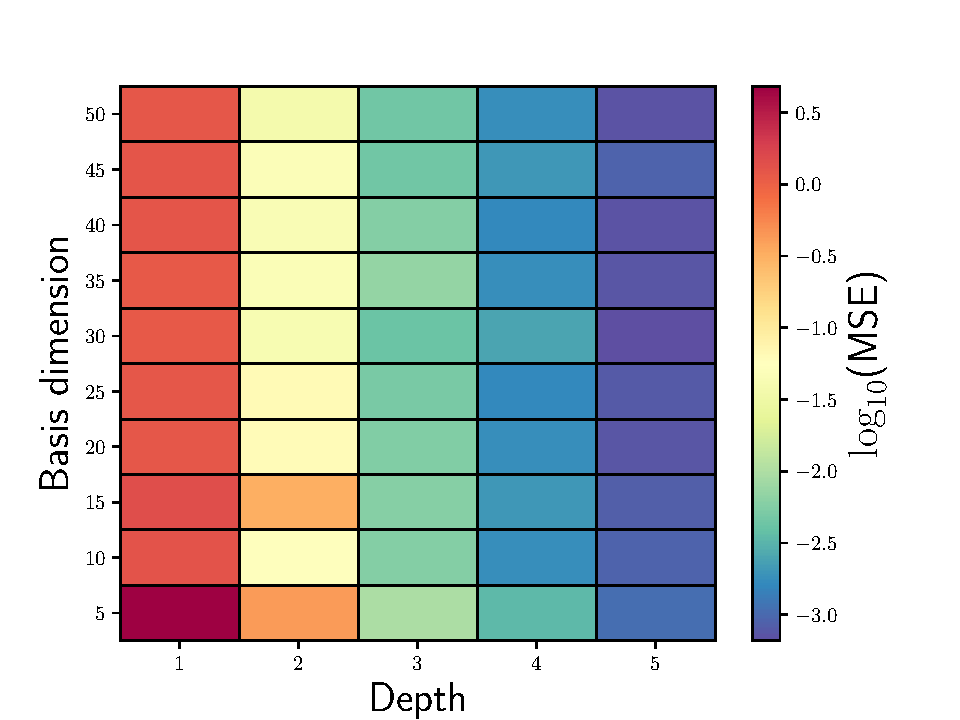
\includegraphics[trim={0cm 0cm 0cm 0cm},clip,width=1.0\linewidth]{code/burgers/synapse_models/basis_study/MSE_training.pdf}
\caption{Least-squares ROM relative error}
\end{subfigure}
\begin{subfigure}[t]{0.49\textwidth}
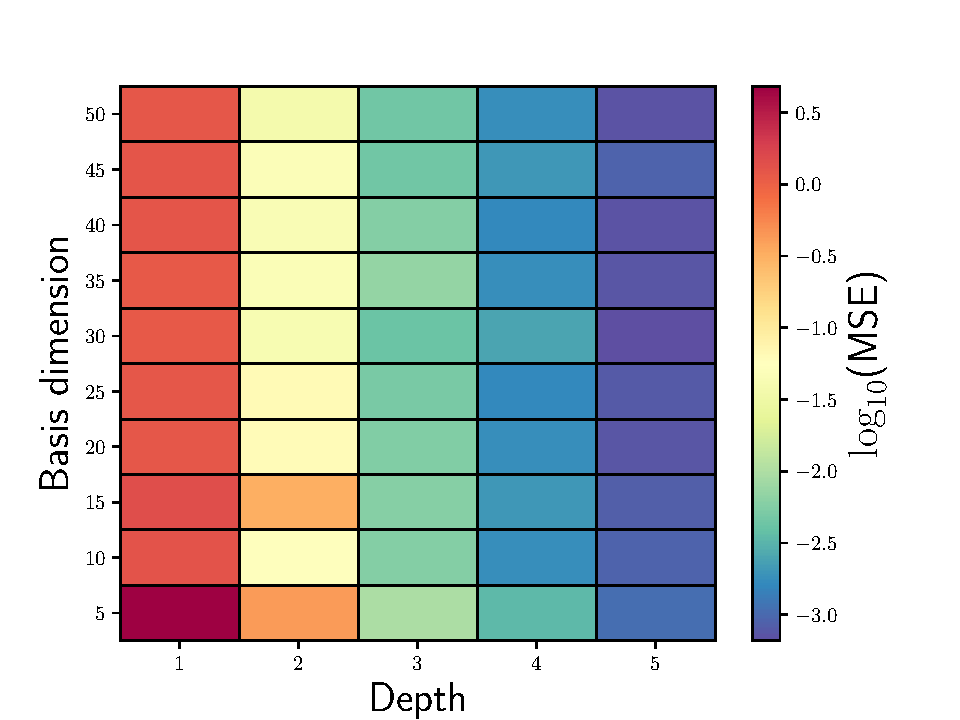
\includegraphics[trim={0cm 0cm 0cm 0cm},clip,width=1.0\linewidth]{code/burgers/synapse_models/basis_study/MSE_training.pdf}
\caption{$\ell^1$ ROM relative error}
\end{subfigure}
\begin{subfigure}[t]{0.49\textwidth}
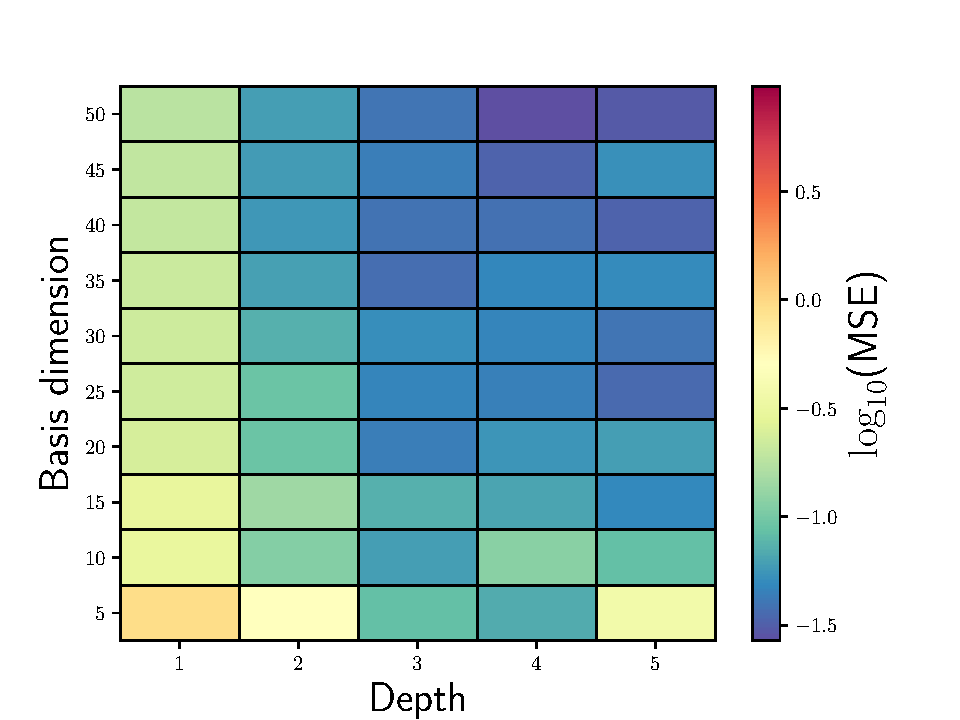
\includegraphics[trim={0cm 0cm 0cm 0cm},clip,width=1.0\linewidth]{code/burgers/synapse_models/basis_study/MSE_testing.pdf}
\caption{Least-squares ROM relative error}
\end{subfigure}
\begin{subfigure}[t]{0.49\textwidth}
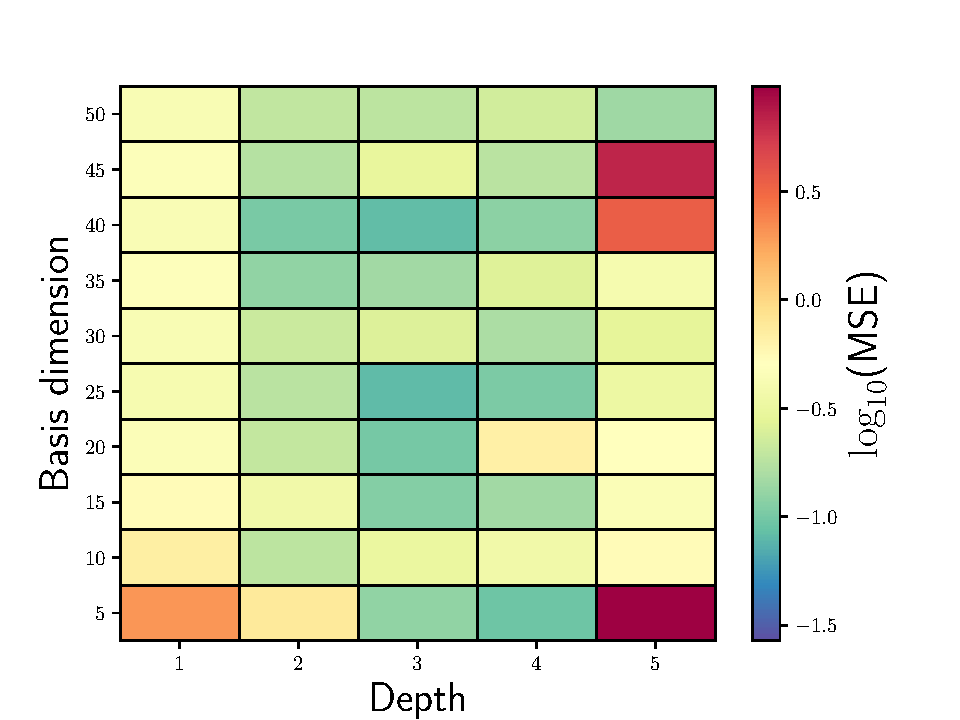
\includegraphics[trim={0cm 0cm 0cm 0cm},clip,width=1.0\linewidth]{code/burgers/synapse_models/basis_study/MSE_testing_ML.pdf}
\caption{$\ell^1$ ROM relative error}
\end{subfigure}
\label{fig:burg_training_results}
\end{center}
\end{figure}

\begin{figure}
\begin{center}
\begin{subfigure}[t]{0.49\textwidth}
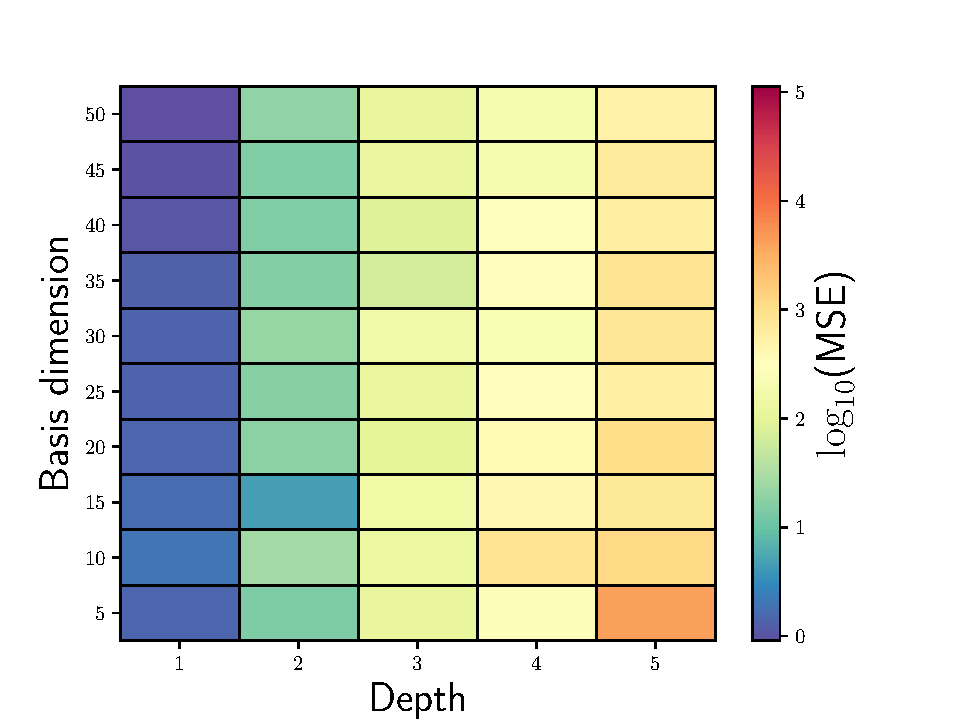
\includegraphics[trim={0cm 0cm 0cm 0cm},clip,width=1.0\linewidth]{code/burgers/synapse_models/basis_study/gen_gap.pdf}
\caption{Least-squares ROM relative error}
\end{subfigure}
\begin{subfigure}[t]{0.49\textwidth}
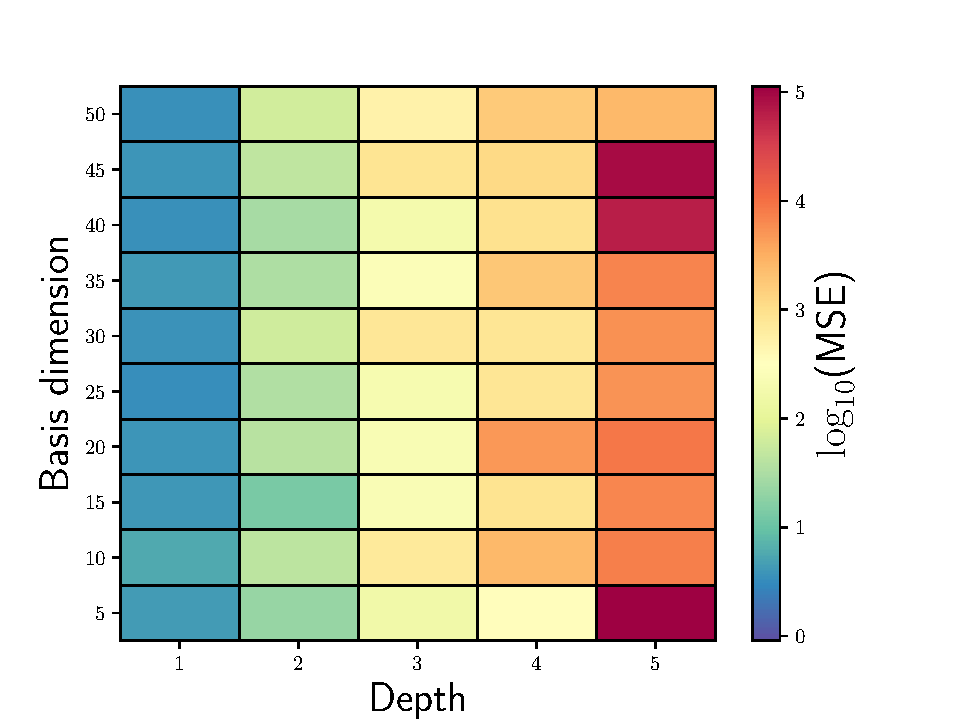
\includegraphics[trim={0cm 0cm 0cm 0cm},clip,width=1.0\linewidth]{code/burgers/synapse_models/basis_study/gen_gap_ML.pdf}
\caption{$\ell^1$ ROM relative error}
\end{subfigure}
\label{fig:burg_training_results}
\end{center}
\end{figure}

\begin{figure}
\begin{center}
\begin{subfigure}[t]{0.49\textwidth}
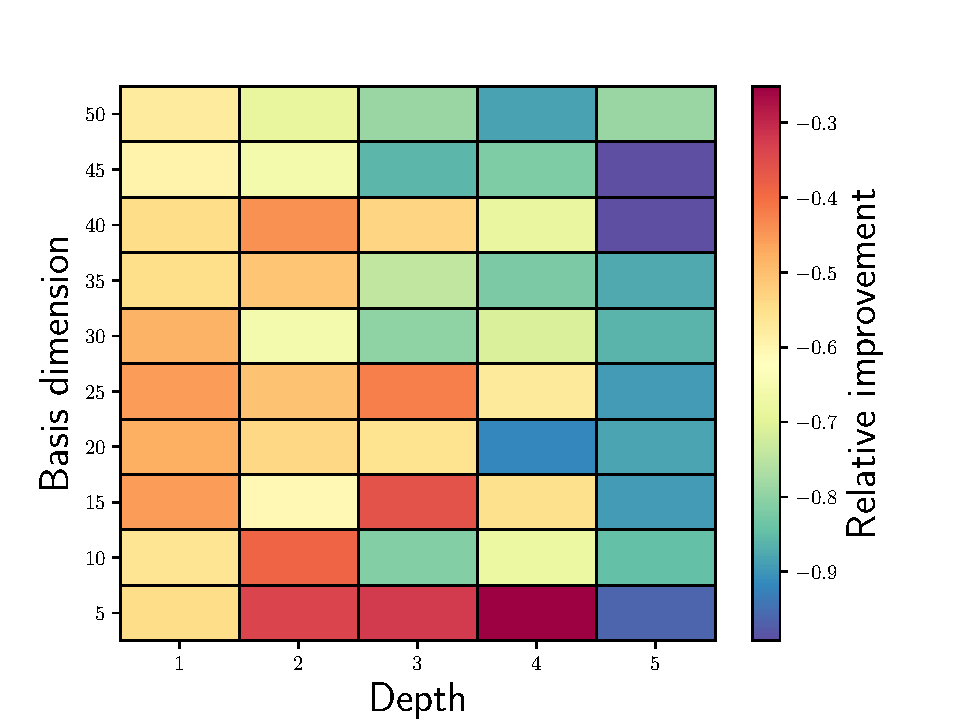
\includegraphics[trim={0cm 0cm 0cm 0cm},clip,width=1.0\linewidth]{code/burgers/synapse_models/basis_study/rel_improvement.pdf}
\caption{Least-squares ROM relative error}
\end{subfigure}
\label{fig:burg_training_results}
\end{center}
\end{figure}



\subsection{Results: Extrapolation in parameter space and time}
We now present results for the framework with both extrapolation in parameter space and in time. We execute reduced-order models on the $8x8$ Cartesian parameter grid  $\mu_1 \times \mu_2 = \{ 4. 0+  \frac{2i}{7} \}_{i=0}^7 \times \{ 0.01 + \frac{j}{70} \}_{j=0}^7$ for $t \in [0,30]$, which comprises extrapolation in both the parameter and temporal dimension. Table~\ref{tab:burg_results} tabulates the mean error and standard deviation for the various ROM methods, where the error and standard deviation are computed from the 5 MLPs. Similarly, Figure~\ref{fig:burg_phys_space} depicts ensembles of physical space solutions for the various ROMs. We observe that all methods are accurate, particularly in the interpolation regime. We observe that, on average, the $\ell^1$ res-min ROM yields the most accurate solutions, followed by the ML and least-squares ROMs. The Galerkin method was only stable for 3 of 5 runs; when stable, Galerkin yields reasonable results, but not as accurate as the other approaches.

Next, Figure~\ref{fig:error_vs_params} presents relative errors averaged over the ensemble for the various ROMs. We observe that all ROMs yield similar results: Sub 1\% relative errors are obtained for all parameters within the training regime, and sub 1.5\% relative errors are obtained for extrapolation cases. We additionally observe that the models extrapolate much better in the $\mu_2$ parameter than in the $\mu_1$ parameter. 
\begin{table}[]
\begin{centering}
\begin{tabular}{l l l l}
\hline
  & $\ell^2$-error  & Residual $\ell^2$-norm & $\ell^2$-error (best) \\
\hline
ML-ROM    & $788.014 \pm 102.694 $ & $35.640 \pm 3.514$  &  $652.778 $ \\
Least-squares ROM & $822.000 \pm 108.855$ & $34.040 \pm 3.004$ & $661.549$\\
$\ell^1$ ROM    & $776.741 \pm 105.274$ &  $35.103 \pm  3.189$ & $652.880$\\
Galerkin ROM    & NA &  NA & $689.189$  \\
\hline
\end{tabular}
\caption{Summary of the various basis sizes employed in the cavity flow example.}
\label{tab:burg_results}
\end{centering}
\end{table}

\begin{figure}
\begin{center}
\begin{subfigure}[t]{0.24\textwidth}
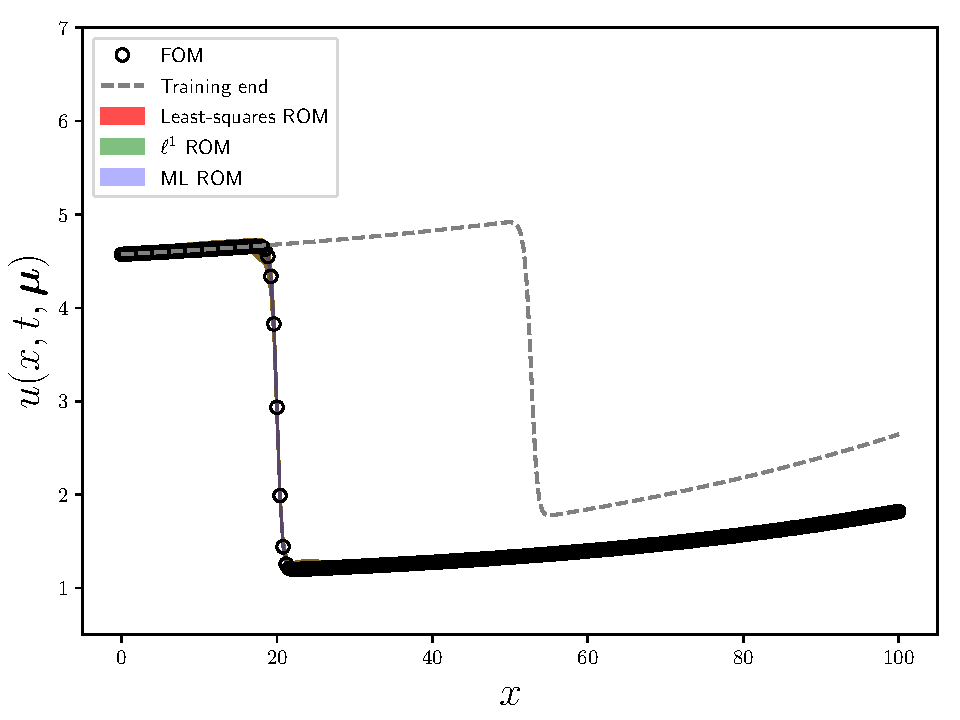
\includegraphics[trim={0cm 0cm 0cm 0cm},clip,width=1.0\linewidth]{code/burgers/synapse_models/elu/results/usol_0001.pdf} 
\caption{$t=7.0$}
\end{subfigure}
\begin{subfigure}[t]{0.24\textwidth}
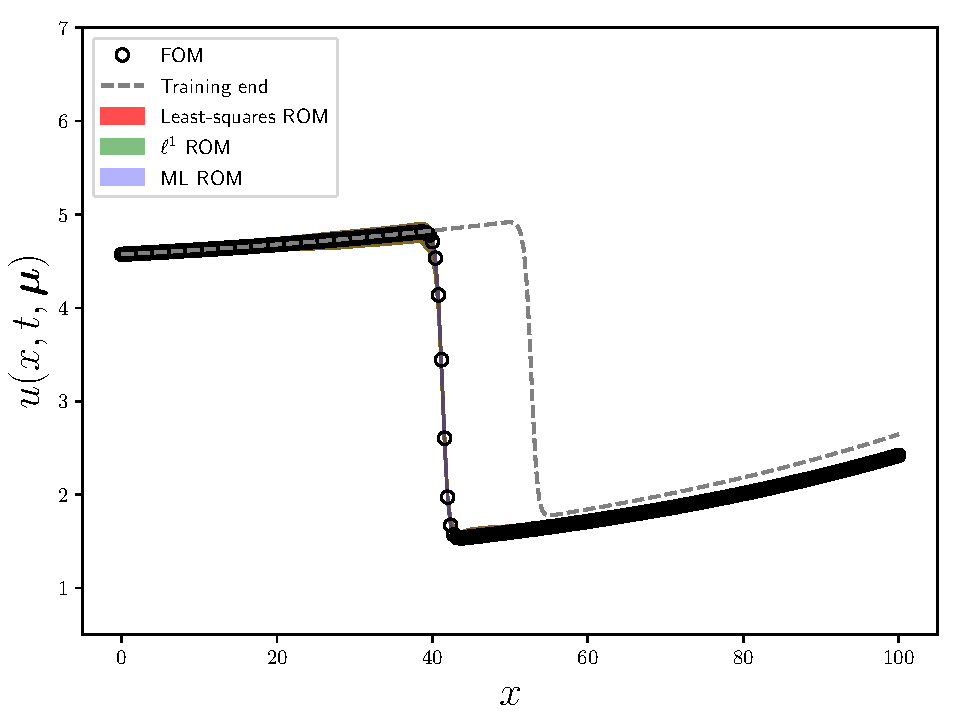
\includegraphics[trim={0cm 0cm 0cm 0cm},clip,width=1.0\linewidth]{code/burgers/synapse_models/elu/results/usol_0003.pdf} 
\caption{$t=10.0$}
\end{subfigure}
\begin{subfigure}[t]{0.24\textwidth}
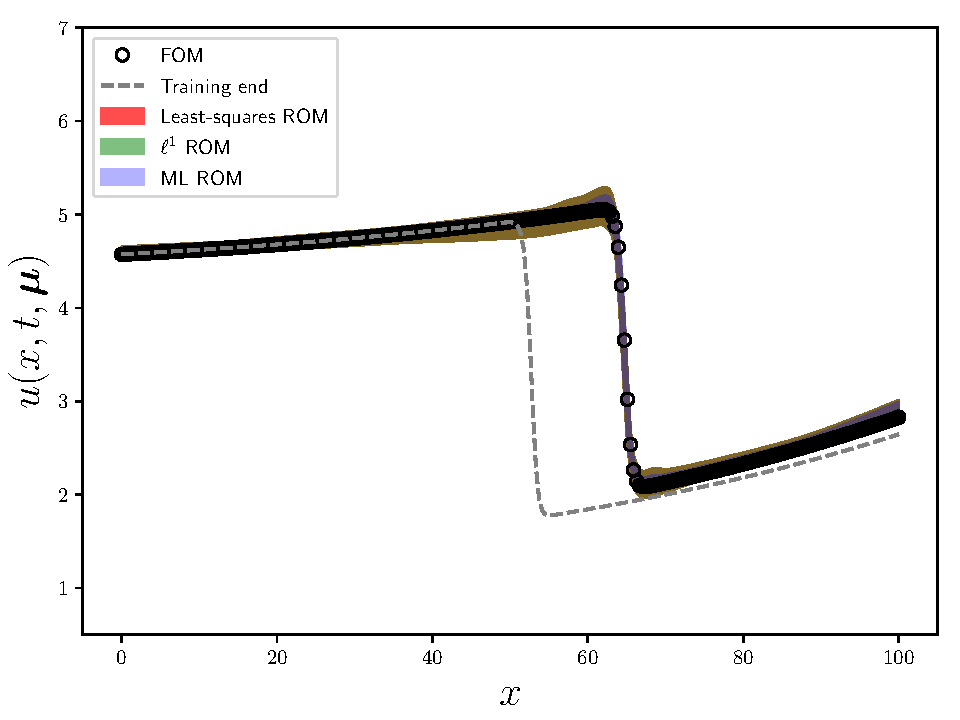
\includegraphics[trim={0cm 0cm 0cm 0cm},clip,width=1.0\linewidth]{code/burgers/synapse_models/elu/results/usol_0005.pdf} 
\caption{$t=21.0$}
\end{subfigure}
\begin{subfigure}[t]{0.24\textwidth}
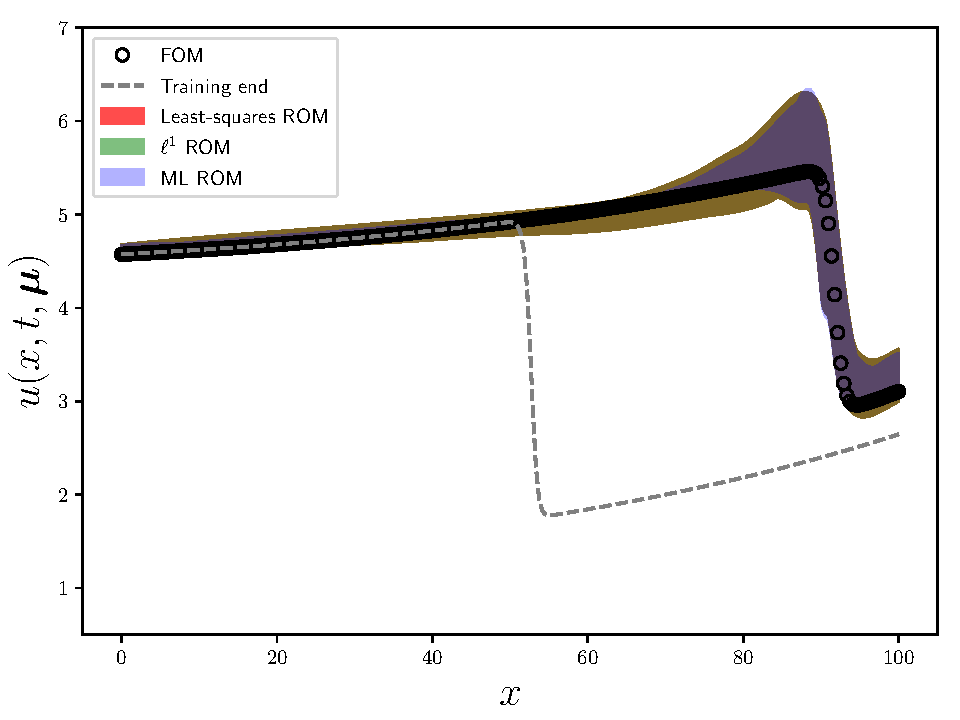
\includegraphics[trim={0cm 0cm 0cm 0cm},clip,width=1.0\linewidth]{code/burgers/synapse_models/elu/results/usol_0007.pdf} 
\caption{$t=28.0$}
\end{subfigure}
\begin{subfigure}[t]{0.24\textwidth}
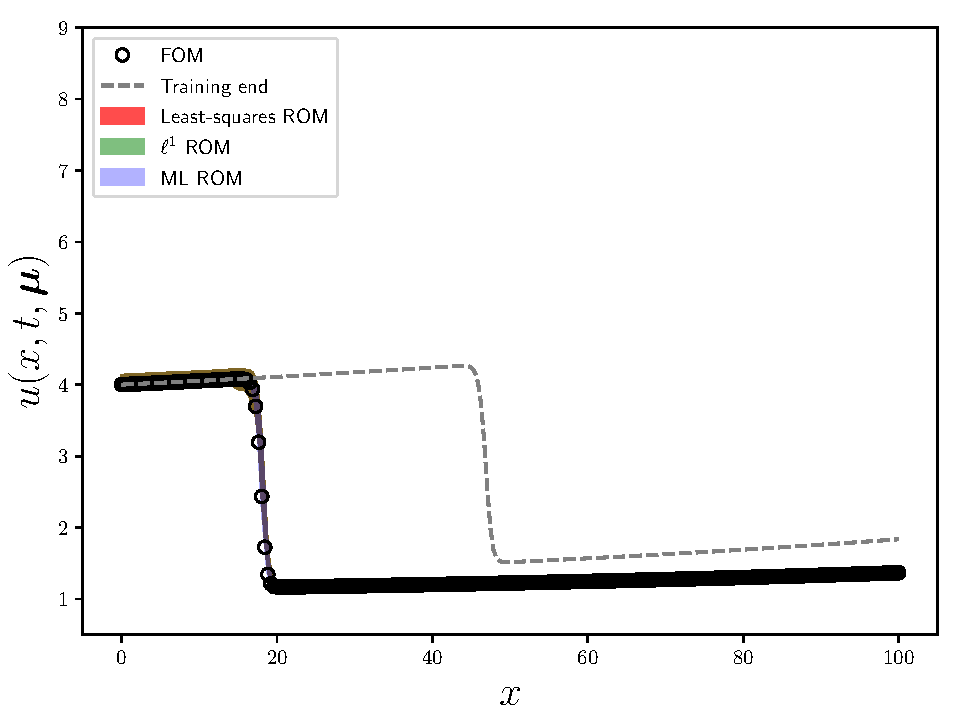
\includegraphics[trim={0cm 0cm 0cm 0cm},clip,width=1.0\linewidth]{code/burgers/synapse_models/elu/results/usolExtrapolate_0001.pdf} 
\caption{$t=7.0$}
\end{subfigure}
\begin{subfigure}[t]{0.24\textwidth}
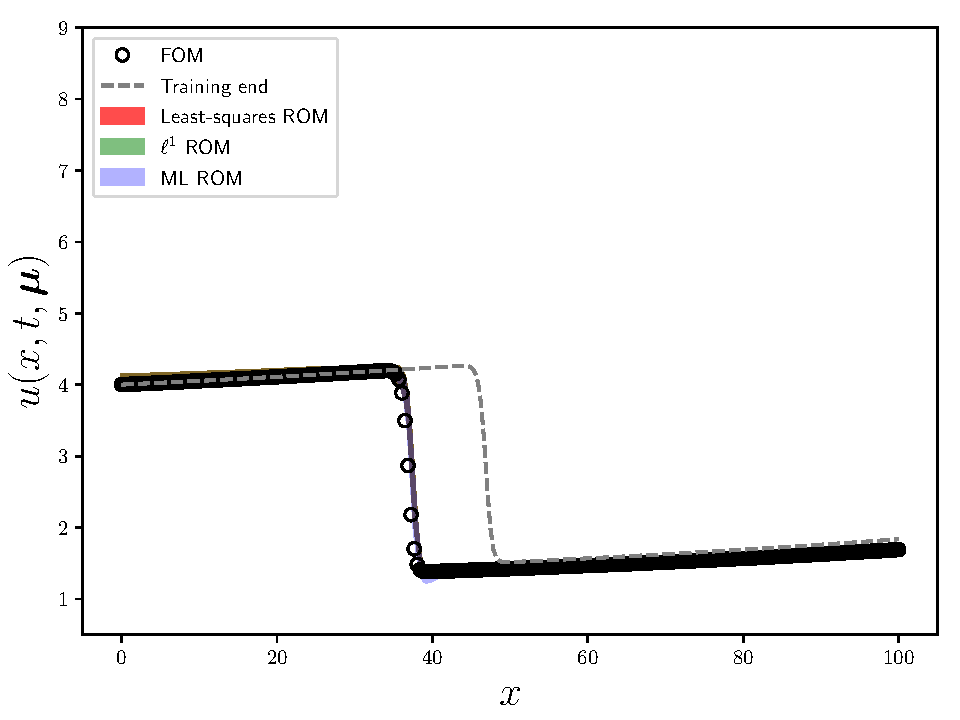
\includegraphics[trim={0cm 0cm 0cm 0cm},clip,width=1.0\linewidth]{code/burgers/synapse_models/elu/results/usolExtrapolate_0003.pdf} 
\caption{$t=10.0$}
\end{subfigure}
\begin{subfigure}[t]{0.24\textwidth}
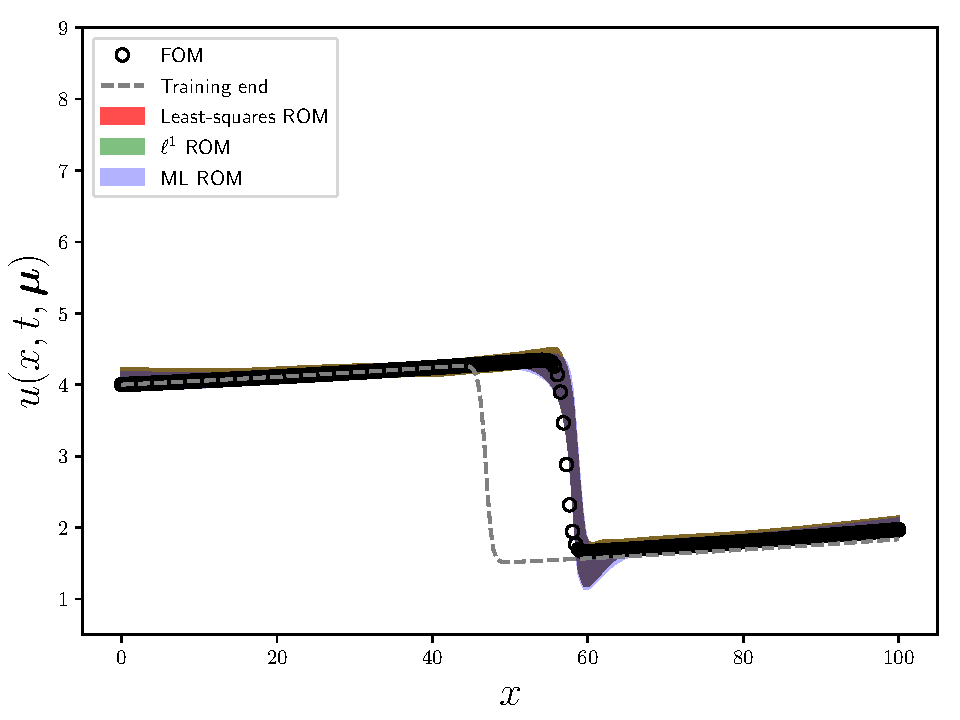
\includegraphics[trim={0cm 0cm 0cm 0cm},clip,width=1.0\linewidth]{code/burgers/synapse_models/elu/results/usolExtrapolate_0005.pdf} 
\caption{$t=21.0$}
\end{subfigure}
\begin{subfigure}[t]{0.24\textwidth}
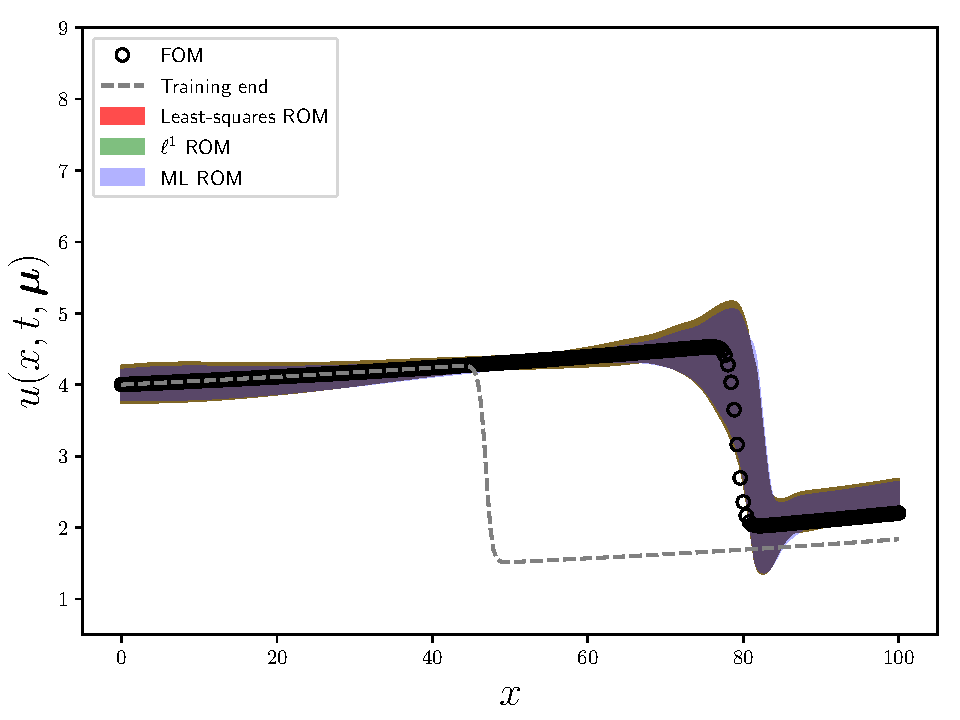
\includegraphics[trim={0cm 0cm 0cm 0cm},clip,width=1.0\linewidth]{code/burgers/synapse_models/elu/results/usolExtrapolate_0007.pdf} 
\caption{$t=28.0$}
\end{subfigure}
\begin{subfigure}[t]{0.24\textwidth}
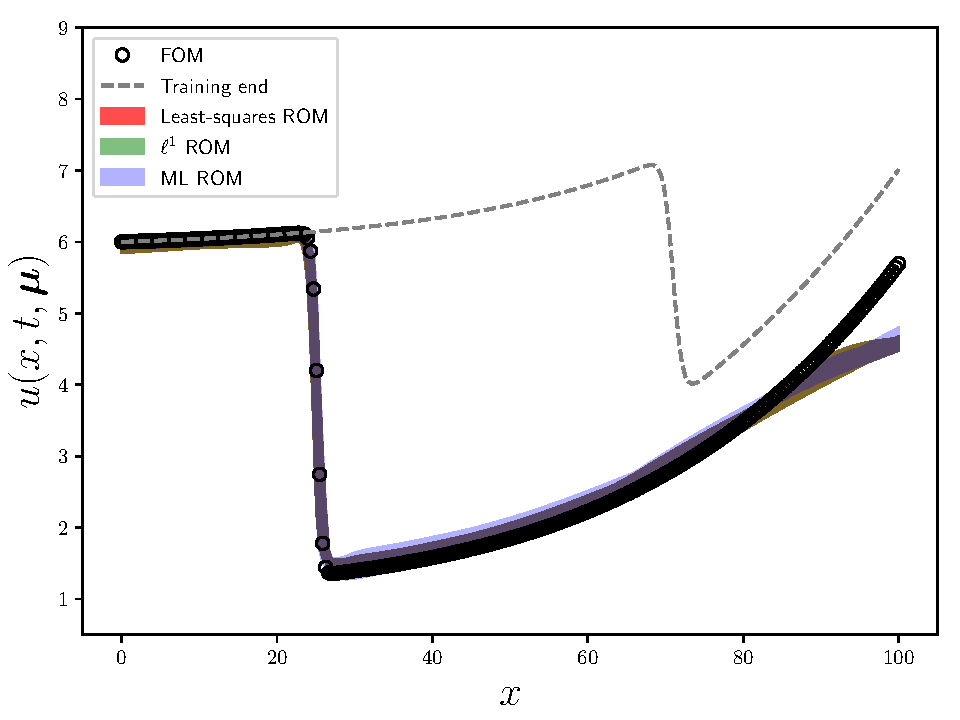
\includegraphics[trim={0cm 0cm 0cm 0cm},clip,width=1.0\linewidth]{code/burgers/synapse_models/elu/results/usolExtrapolate2_0001.pdf} 
\caption{$t=7.0$}
\end{subfigure}
\begin{subfigure}[t]{0.24\textwidth}
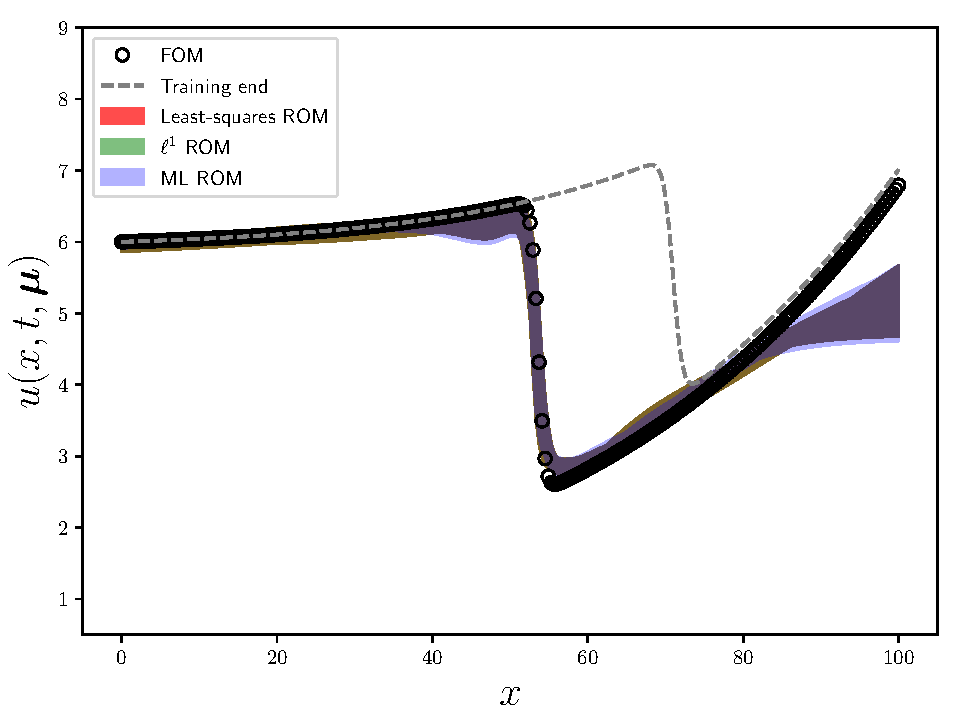
\includegraphics[trim={0cm 0cm 0cm 0cm},clip,width=1.0\linewidth]{code/burgers/synapse_models/elu/results/usolExtrapolate2_0003.pdf} 
\caption{$t=10.0$}
\end{subfigure}
\begin{subfigure}[t]{0.24\textwidth}
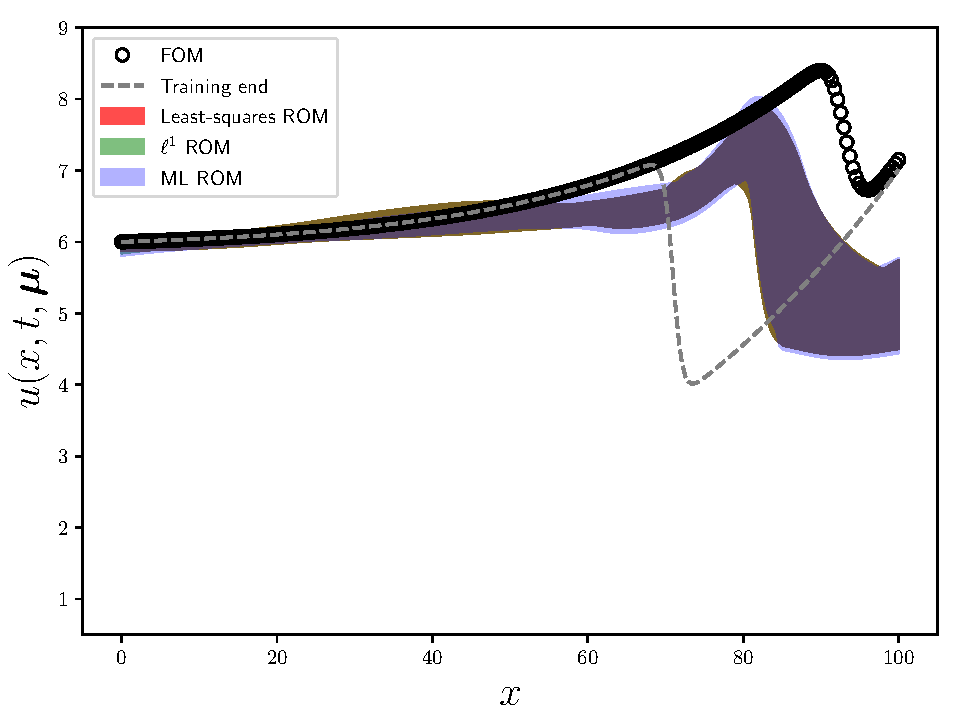
\includegraphics[trim={0cm 0cm 0cm 0cm},clip,width=1.0\linewidth]{code/burgers/synapse_models/elu/results/usolExtrapolate2_0005.pdf} 
\caption{$t=21.0$}
\end{subfigure}
\begin{subfigure}[t]{0.24\textwidth}
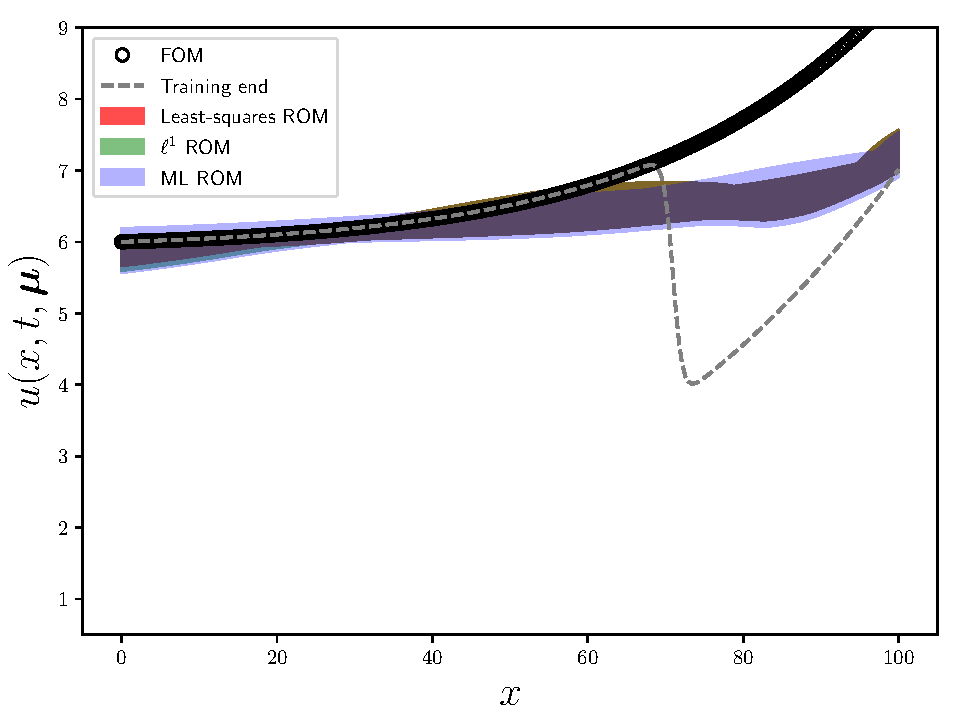
\includegraphics[trim={0cm 0cm 0cm 0cm},clip,width=1.0\linewidth]{code/burgers/synapse_models/elu/results/usolExtrapolate2_0007.pdf} 
\caption{$t=28.0$}
\end{subfigure}

\caption{Physical solutions for ROMs of the 1D Burgers equation at various time instances. Parameter interpolation (top), and parameter extrapolation (bottom).}
\label{fig:burg_phys_space}
\end{center}
\end{figure}

\begin{figure}
\begin{center}
\begin{subfigure}[t]{0.32\textwidth}
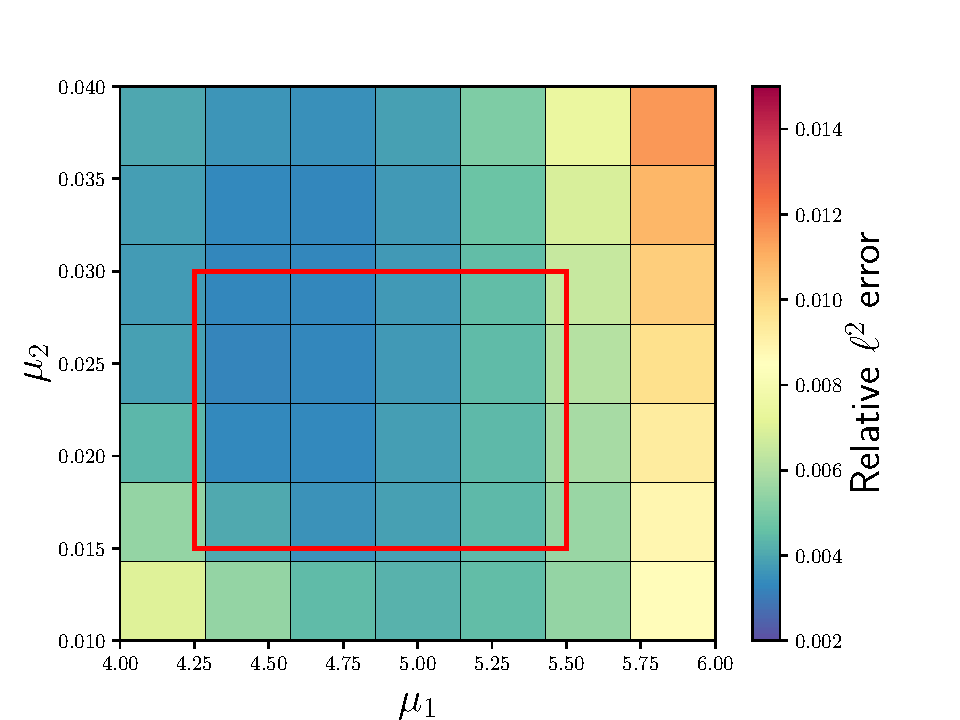
\includegraphics[trim={0cm 0cm 0cm 0cm},clip,width=1.0\linewidth]{code/burgers/synapse_models/elu/results/uls_error_vs_param.pdf} 
\caption{Least-squares ROM relative error}
\end{subfigure}
\begin{subfigure}[t]{0.32\textwidth}
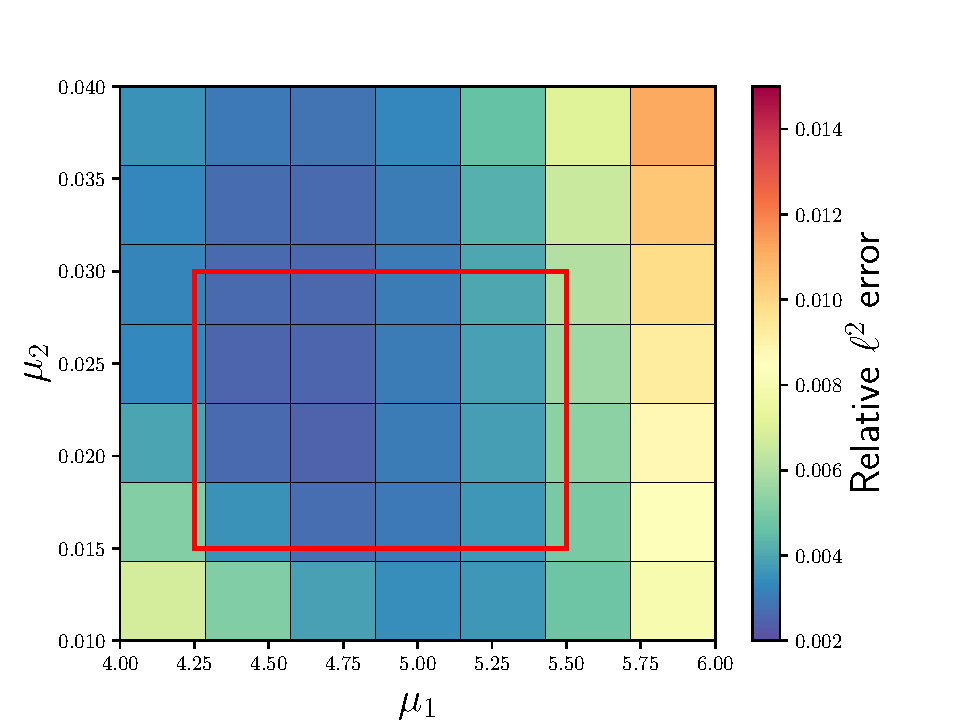
\includegraphics[trim={0cm 0cm 0cm 0cm},clip,width=1.0\linewidth]{code/burgers/synapse_models/elu/results/ul1_error_vs_param.pdf} 
\caption{$\ell^1$ ROM relative error}
\end{subfigure}
\begin{subfigure}[t]{0.32\textwidth}
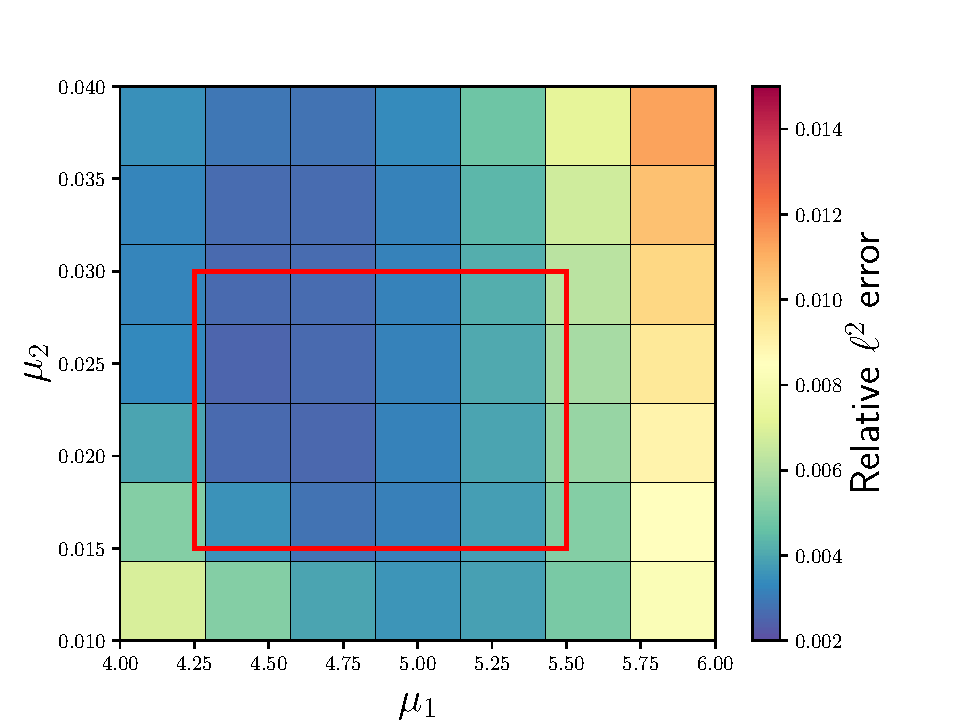
\includegraphics[trim={0cm 0cm 0cm 0cm},clip,width=1.0\linewidth]{code/burgers/synapse_models/elu/results/uml_error_vs_param.pdf} 
\caption{ML ROM relative error}
\end{subfigure}
\label{fig:rom_metrics_swe_updatefreq}
\end{center}
\end{figure}

\bibliographystyle{siam}
\bibliography{refs}

\end{document}

